%%=============================================================================
%% LaTeX sjabloon voor bachelorproef, HoGent Bedrijf en Organisatie
%% Opleiding Toegepaste Informatica
%%=============================================================================

\documentclass[fleqn,a4paper,12pt]{book}

%%=============================================================================
%% LaTeX sjabloon voor de bachelorproef, HoGent Bedrijf en Organisatie
%% Opleiding toegepaste informatica
%%
%% Structuur en algemene vormgeving. Meestal hoef je hier niets te wijzigen.
%%
%% Vormgeving gebaseerd op "The Legrand Orange Book", version 2.0 (9/2/15)
%% door Mathias Legrand (legrand.mathias@gmail.com) met aanpassingen door
%% Vel (vel@latextemplates.com). Het oorspronkelijke template is te vinden op
%% http://www.LaTeXTemplates.com
%%
%% Aanpassingen voor HoGent toegepaste informatica: 
%%   Bert Van Vreckem <bert.vanvreckem@hogent.be>
%% Licentie: 
%%   CC BY-NC-SA 3.0 (http://creativecommons.org/licenses/by-nc-sa/3.0/)
%%=============================================================================

%%-----------------------------------------------------------------------------
%% Packages
%%-----------------------------------------------------------------------------

\usepackage[top=3cm,bottom=3cm,left=3cm,right=3cm,headsep=10pt,a4paper]{geometry} % Page margins
\usepackage[utf8]{inputenc}  % Accenten gebruiken in tekst (vb. é ipv \'e)
\usepackage{amsfonts}        % AMS math packages: extra wiskundige
\usepackage{amsmath}         %   symbolen (o.a. getallen-
\usepackage{amssymb}         %   verzamelingen N, R, Z, Q, etc.)
\usepackage[english,dutch]{babel}    % Taalinstellingen: woordsplitsingen,
                             %  commando's voor speciale karakters
                             %  ("dutch" voor NL)
\usepackage{iflang}
\usepackage{eurosym}         % Euro-symbool €
\usepackage{geometry}
\usepackage{graphicx}        % Invoegen van tekeningen
\graphicspath{{img/}}       % Specifies the directory where pictures are stored
\usepackage{tikz}            % Required for drawing custom shapes
\usepackage[pdftex,bookmarks=true]{hyperref}
                             % PDF krijgt klikbare links & verwijzingen,
                             %  inhoudstafel
\usepackage{enumitem}        % Customize lists
\setlist{nolistsep}         % Reduce spacing between list items
\usepackage{listings}        % Broncode mooi opmaken
\usepackage{multirow}        % Tekst over verschillende cellen in tabellen
\usepackage{rotating}        % Tabellen en figuren roteren

\usepackage{booktabs}        % Required for nicer horizontal rules in tables

\usepackage{xcolor}          % Required for specifying colors by name
\definecolor{maincolor}{RGB}{0,147,208} % Define the main color used for 
                             % highlighting throughout the book
                             % 0, 147, 208 = officiële kleur HoGent FBO

% Paragraph style: no indent, add space between paragraphs
\setlength{\parindent}{0em}
\setlength{\parskip}{1em}

\usepackage{etoolbox}
\usepackage{titling} % Macros for title, author, etc
\usepackage{lipsum}          % Voor vultekst (lorem ipsum)

%----------------------------------------------------------------------------------------
%	FONTS
%----------------------------------------------------------------------------------------

\usepackage{avant} % Use the Avantgarde font for headings
%\usepackage{times} % Use the Times font for headings
\usepackage{mathptmx} % Use the Adobe Times Roman as the default text font together with math symbols from the Sym­bol, Chancery and Com­puter Modern fonts

\usepackage{microtype} % Slightly tweak font spacing for aesthetics
\usepackage[utf8]{inputenc} % Required for including letters with accents
\usepackage[T1]{fontenc} % Use 8-bit encoding that has 256 glyphs

%------------------------------------------------------------------------------
%	TITLE PAGE
%------------------------------------------------------------------------------

\newcommand{\inserttitlepage}{%
\begin{titlepage}
  \newgeometry{top=2cm,bottom=1.5cm,left=1.5cm,right=1.5cm}
  \begin{center}

    \begingroup
    \rmfamily
    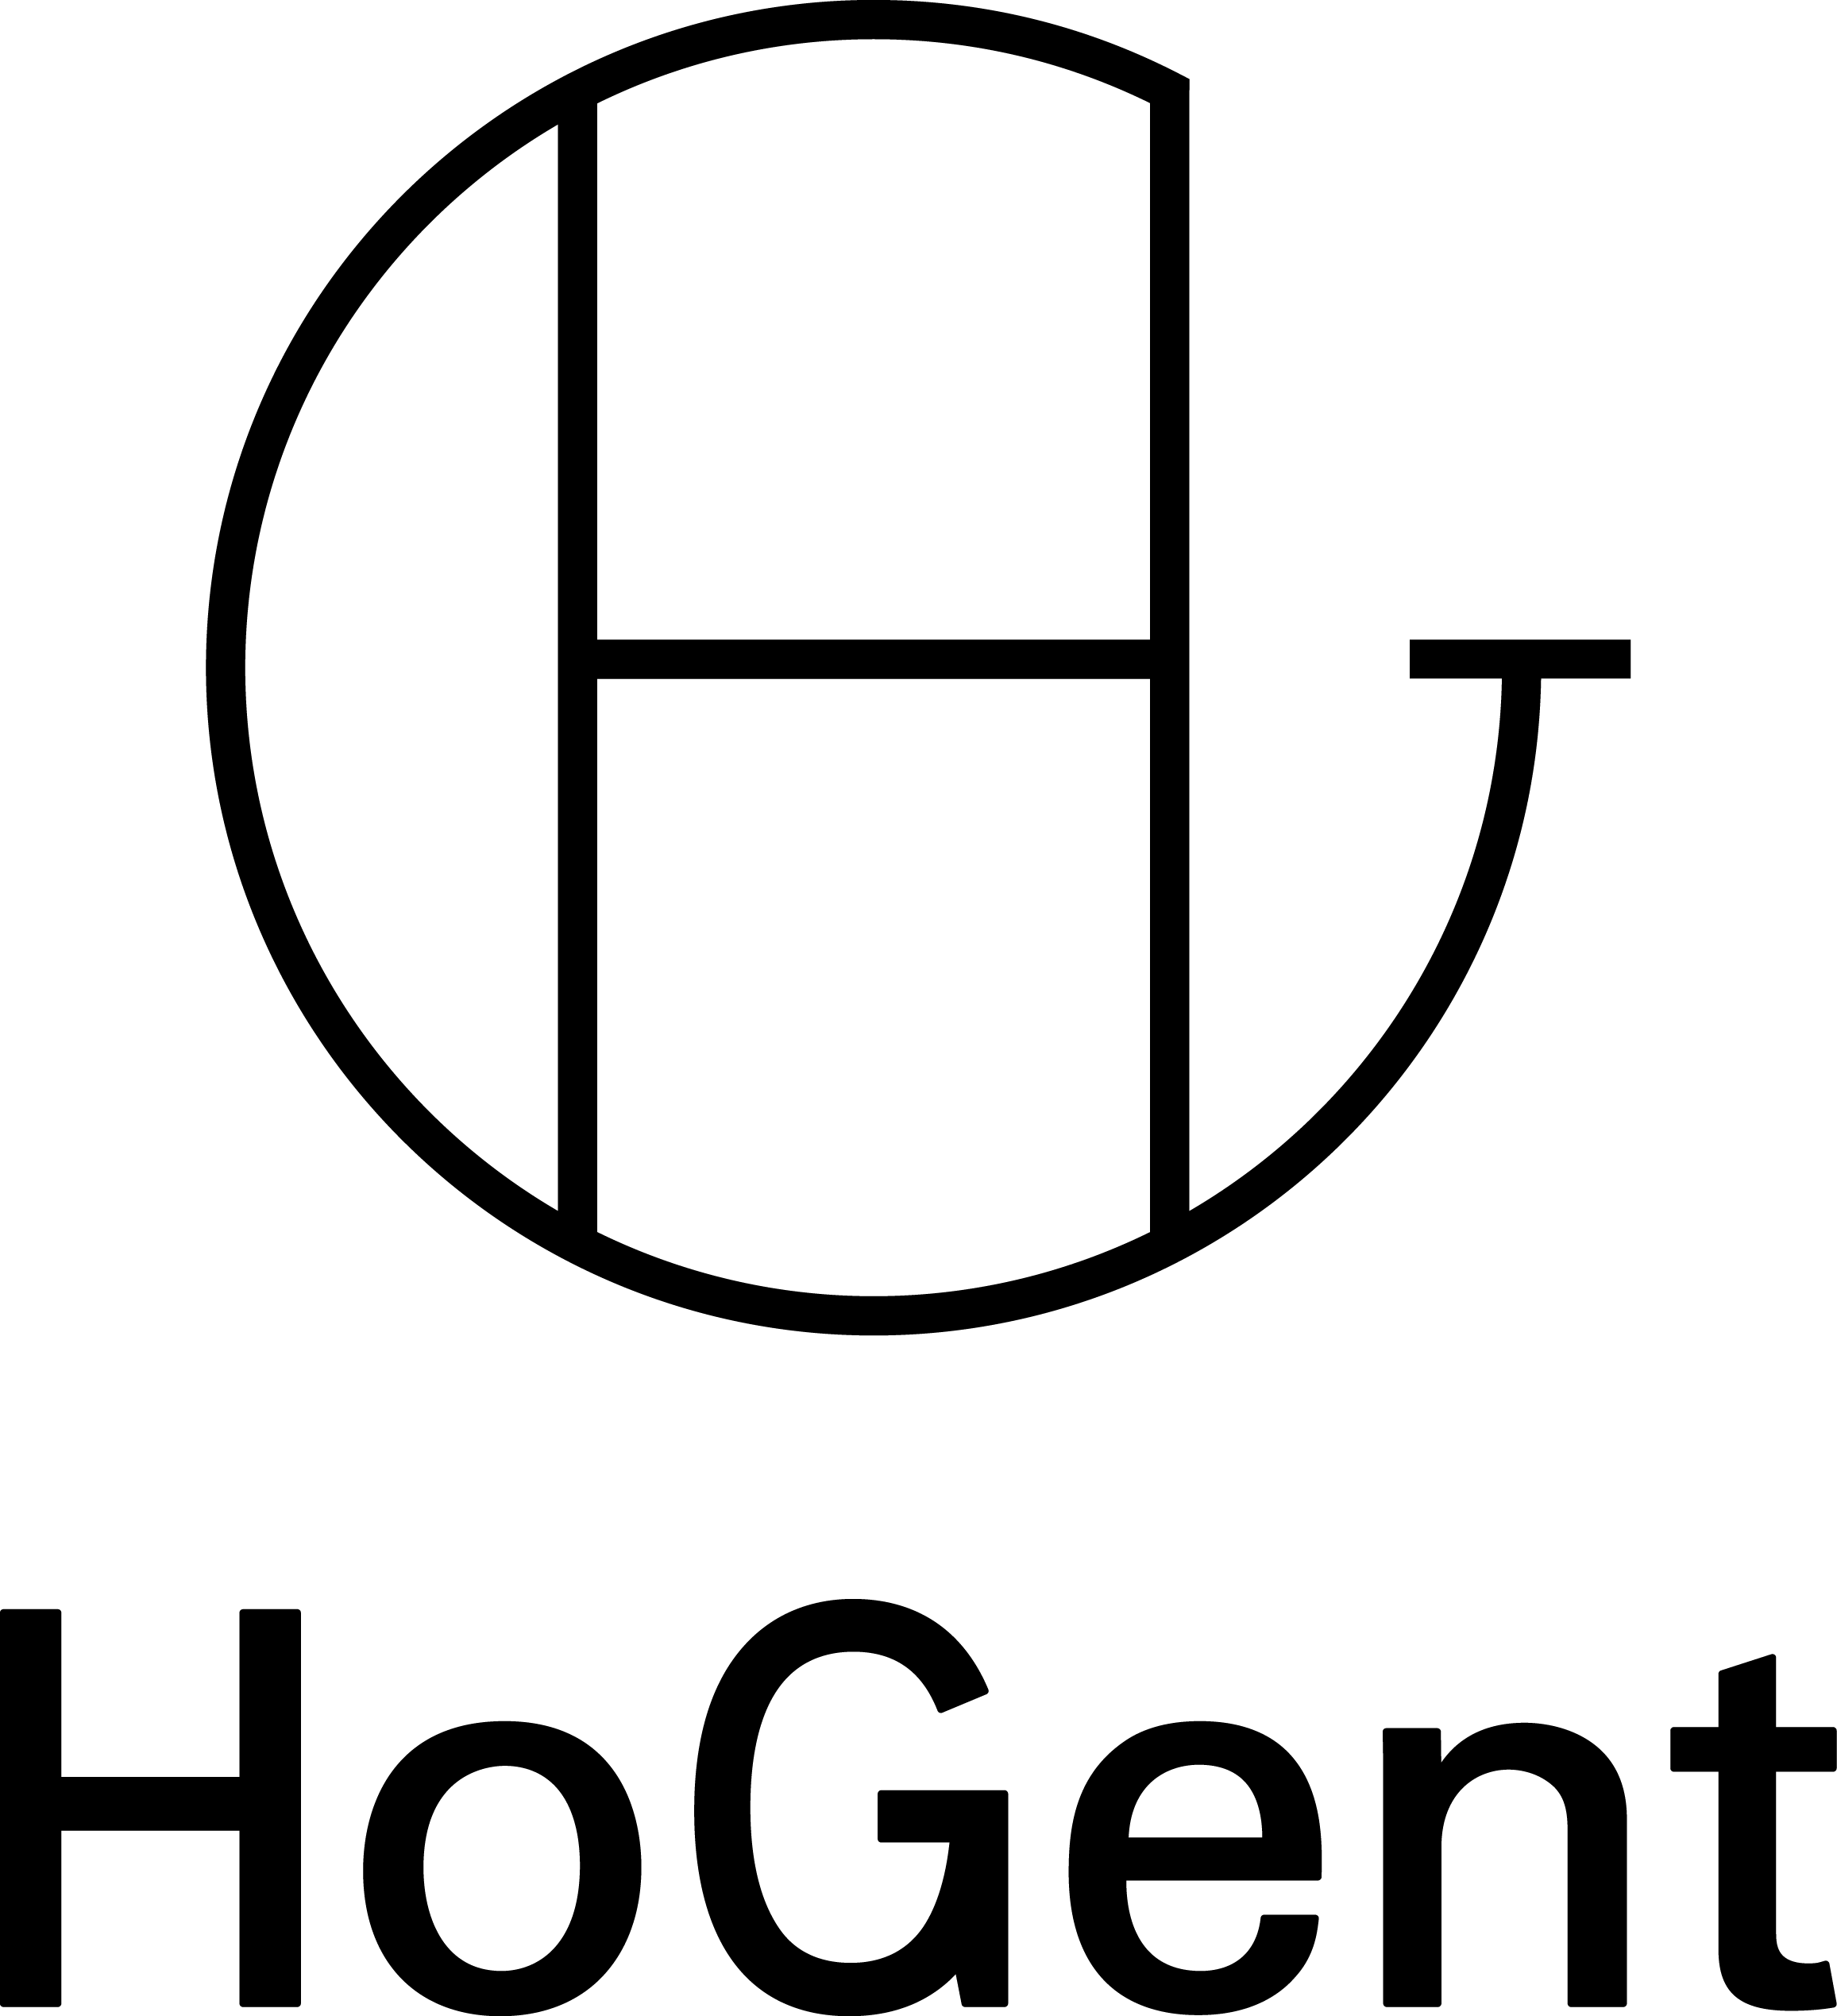
\includegraphics[width=2.5cm]{img/HG-beeldmerk-woordmerk}\\[.5cm]
    Faculteit Bedrijf en Organisatie\\[3cm]
    \titel
    \vfill
    \student\\[3.5cm]
    Scriptie voorgedragen tot het bekomen van de graad van\\professionele bachelor in de toegepaste informatica\\[2cm]
    Promotor:\\
    \promotor\\
    \ifdefempty{\copromotor}{\vspace{2.5cm}}{Co-promotor:\\\copromotor\\[2.5cm]}
    Instelling: \instelling\\[.5cm]
    Academiejaar: \academiejaar\\[.5cm]
    \ifcase \examenperiode \or Eerste \or Tweede \else Derde \fi examenperiode
    \endgroup

  \end{center}
  \restoregeometry
\end{titlepage}
  \emptypage
\begin{titlepage}
  \newgeometry{top=5.35cm,bottom=1.5cm,left=1.5cm,right=1.5cm}
  \begin{center}

    \begingroup
    \rmfamily
    \IfLanguageName{dutch}{Faculteit Bedrijf en Organisatie}{Faculty of Business and Information Management}\\[3cm]
    \titel
    \vfill
    \student\\[3.5cm]
    \IfLanguageName{dutch}{Scriptie voorgedragen tot het bekomen van de graad van\\professionele bachelor in de toegepaste informatica}{Thesis submitted in partial fulfilment of the requirements for the degree of\\professional bachelor of applied computer science}\\[2cm]
    Promotor:\\
    \promotor\\
    \ifdefempty{\copromotor}{\vspace{2.5cm}}{Co-promotor:\\\copromotor\\[2.5cm]}
    \IfLanguageName{dutch}{Instelling}{Institution}: \instelling\\[.5cm]
    \IfLanguageName{dutch}{Academiejaar}{Academic year}: \academiejaar\\[.5cm]
    \IfLanguageName{dutch}{%
    \ifcase \examenperiode \or Eerste \or Tweede \else Derde \fi examenperiode}{%
    \ifcase \examenperiode \or First \or Second \else Third \fi examination period}
    \endgroup

  \end{center}
  \restoregeometry
\end{titlepage}
}

%----------------------------------------------------------------------------------------
%	BIBLIOGRAPHY AND INDEX
%----------------------------------------------------------------------------------------

\usepackage[style=apa,backend=biber]{biblatex}
\usepackage{csquotes}
\DeclareLanguageMapping{dutch}{dutch-apa}
\addbibresource{bachproef-tin.bib} % BibTeX bibliography file
\addbibresource{../voorstel/voorstel.bib}
\defbibheading{bibempty}{}

\usepackage{calc} % For simpler calculation - used for spacing the index letter headings correctly
\usepackage{makeidx} % Required to make an index
\makeindex % Tells LaTeX to create the files required for indexing

%----------------------------------------------------------------------------------------
%	MAIN TABLE OF CONTENTS
%----------------------------------------------------------------------------------------

\usepackage{titletoc} % Required for manipulating the table of contents

\contentsmargin{0cm} % Removes the default margin

% Part text styling
\titlecontents{part}[0cm]
{\addvspace{20pt}\centering\large\bfseries}
{}
{}
{}

% Chapter text styling
\titlecontents{chapter}[1.25cm] % Indentation
{\addvspace{12pt}\large\sffamily\bfseries} % Spacing and font options for chapters
{\color{maincolor!60}\contentslabel[\Large\thecontentslabel]{1.25cm}\color{maincolor}} % Chapter number
{\color{maincolor}}
{\color{maincolor!60}\normalsize\;\titlerule*[.5pc]{.}\;\thecontentspage} % Page number

% Section text styling
\titlecontents{section}[1.25cm] % Indentation
{\addvspace{3pt}\sffamily\bfseries} % Spacing and font options for sections
{\contentslabel[\thecontentslabel]{1.25cm}} % Section number
{}
{\hfill\color{black}\thecontentspage} % Page number
[]

% Subsection text styling
\titlecontents{subsection}[1.25cm] % Indentation
{\addvspace{1pt}\sffamily\small} % Spacing and font options for subsections
{\contentslabel[\thecontentslabel]{1.25cm}} % Subsection number
{}
{\ \titlerule*[.5pc]{.}\;\thecontentspage} % Page number
[]

% List of figures
\titlecontents{figure}[0em]
{\addvspace{-5pt}\sffamily}
{\thecontentslabel\hspace*{1em}}
{}
{\ \titlerule*[.5pc]{.}\;\thecontentspage}
[]

% List of tables
\titlecontents{table}[0em]
{\addvspace{-5pt}\sffamily}
{\thecontentslabel\hspace*{1em}}
{}
{\ \titlerule*[.5pc]{.}\;\thecontentspage}
[]

%----------------------------------------------------------------------------------------
%	MINI TABLE OF CONTENTS IN PART HEADS
%----------------------------------------------------------------------------------------

% Chapter text styling
\titlecontents{lchapter}[0em] % Indenting
{\addvspace{15pt}\large\sffamily\bfseries} % Spacing and font options for chapters
{\color{maincolor}\contentslabel[\Large\thecontentslabel]{1.25cm}\color{maincolor}} % Chapter number
{}
{\color{maincolor}\normalsize\sffamily\bfseries\;\titlerule*[.5pc]{.}\;\thecontentspage} % Page number

% Section text styling
\titlecontents{lsection}[0em] % Indenting
{\sffamily\small} % Spacing and font options for sections
{\contentslabel[\thecontentslabel]{1.25cm}} % Section number
{}
{}

% Subsection text styling
\titlecontents{lsubsection}[.5em] % Indentation
{\normalfont\footnotesize\sffamily} % Font settings
{}
{}
{}

%----------------------------------------------------------------------------------------
%	PAGE HEADERS
%----------------------------------------------------------------------------------------

\usepackage{fancyhdr} % Required for header and footer configuration

\pagestyle{fancy}
\renewcommand{\chaptermark}[1]{\markboth{\sffamily\normalsize\bfseries\chaptername\ \thechapter.\ #1}{}} % Chapter text font settings
\renewcommand{\sectionmark}[1]{\markright{\sffamily\normalsize\thesection\hspace{5pt}#1}{}} % Section text font settings
\fancyhf{} \fancyhead[LE,RO]{\sffamily\normalsize\thepage} % Font setting for the page number in the header
\fancyhead[LO]{\rightmark} % Print the nearest section name on the left side of odd pages
\fancyhead[RE]{\leftmark} % Print the current chapter name on the right side of even pages
\renewcommand{\headrulewidth}{0.5pt} % Width of the rule under the header
\addtolength{\headheight}{2.5pt} % Increase the spacing around the header slightly
\renewcommand{\footrulewidth}{0pt} % Removes the rule in the footer
\fancypagestyle{plain}{\fancyhead{}\renewcommand{\headrulewidth}{0pt}} % Style for when a plain pagestyle is specified

% Removes the header from odd empty pages at the end of chapters
\makeatletter
\renewcommand{\cleardoublepage}{
\clearpage\ifodd\c@page\else
\hbox{}
\vspace*{\fill}
\thispagestyle{empty}
\newpage
\fi}

%----------------------------------------------------------------------------------------
%	THEOREM STYLES
%----------------------------------------------------------------------------------------

\usepackage{amsmath,amsfonts,amssymb,amsthm} % For math equations, theorems, symbols, etc

\newcommand{\intoo}[2]{\mathopen{]}#1\,;#2\mathclose{[}}
\newcommand{\ud}{\mathop{\mathrm{{}d}}\mathopen{}}
\newcommand{\intff}[2]{\mathopen{[}#1\,;#2\mathclose{]}}
\newtheorem{notation}{Notation}[chapter]

% Boxed/framed environments
\newtheoremstyle{maincolornumbox}% % Theorem style name
{0pt}% Space above
{0pt}% Space below
{\normalfont}% % Body font
{}% Indent amount
{\small\bf\sffamily\color{maincolor}}% % Theorem head font
{\;}% Punctuation after theorem head
{0.25em}% Space after theorem head
{\small\sffamily\color{maincolor}\thmname{#1}\nobreakspace\thmnumber{\@ifnotempty{#1}{}\@upn{#2}}% Theorem text (e.g. Theorem 2.1)
\thmnote{\nobreakspace\the\thm@notefont\sffamily\bfseries\color{black}---\nobreakspace#3.}} % Optional theorem note
\renewcommand{\qedsymbol}{$\blacksquare$}% Optional qed square

\newtheoremstyle{blacknumex}% Theorem style name
{5pt}% Space above
{5pt}% Space below
{\normalfont}% Body font
{} % Indent amount
{\small\bf\sffamily}% Theorem head font
{\;}% Punctuation after theorem head
{0.25em}% Space after theorem head
{\small\sffamily{\tiny\ensuremath{\blacksquare}}\nobreakspace\thmname{#1}\nobreakspace\thmnumber{\@ifnotempty{#1}{}\@upn{#2}}% Theorem text (e.g. Theorem 2.1)
\thmnote{\nobreakspace\the\thm@notefont\sffamily\bfseries---\nobreakspace#3.}}% Optional theorem note

\newtheoremstyle{blacknumbox} % Theorem style name
{0pt}% Space above
{0pt}% Space below
{\normalfont}% Body font
{}% Indent amount
{\small\bf\sffamily}% Theorem head font
{\;}% Punctuation after theorem head
{0.25em}% Space after theorem head
{\small\sffamily\thmname{#1}\nobreakspace\thmnumber{\@ifnotempty{#1}{}\@upn{#2}}% Theorem text (e.g. Theorem 2.1)
\thmnote{\nobreakspace\the\thm@notefont\sffamily\bfseries---\nobreakspace#3.}}% Optional theorem note

% Non-boxed/non-framed environments
\newtheoremstyle{maincolornum}% % Theorem style name
{5pt}% Space above
{5pt}% Space below
{\normalfont}% % Body font
{}% Indent amount
{\small\bf\sffamily\color{maincolor}}% % Theorem head font
{\;}% Punctuation after theorem head
{0.25em}% Space after theorem head
{\small\sffamily\color{maincolor}\thmname{#1}\nobreakspace\thmnumber{\@ifnotempty{#1}{}\@upn{#2}}% Theorem text (e.g. Theorem 2.1)
\thmnote{\nobreakspace\the\thm@notefont\sffamily\bfseries\color{black}---\nobreakspace#3.}} % Optional theorem note
\renewcommand{\qedsymbol}{$\blacksquare$}% Optional qed square
\makeatother

% Defines the theorem text style for each type of theorem to one of the three styles above
\newcounter{dummy}
\numberwithin{dummy}{section}
\theoremstyle{maincolornumbox}
\newtheorem{theoremeT}[dummy]{Theorem}
\newtheorem{problem}{Problem}[chapter]
\newtheorem{exerciseT}{Exercise}[chapter]
\theoremstyle{blacknumex}
\newtheorem{exampleT}{Example}[chapter]
\theoremstyle{blacknumbox}
\newtheorem{vocabulary}{Vocabulary}[chapter]
\newtheorem{definitionT}{Definition}[section]
\newtheorem{corollaryT}[dummy]{Corollary}
\theoremstyle{maincolornum}
\newtheorem{proposition}[dummy]{Proposition}

%----------------------------------------------------------------------------------------
%	DEFINITION OF COLORED BOXES
%----------------------------------------------------------------------------------------

\RequirePackage[framemethod=default]{mdframed} % Required for creating the theorem, definition, exercise and corollary boxes

% Theorem box
\newmdenv[skipabove=7pt,
skipbelow=7pt,
backgroundcolor=black!5,
linecolor=maincolor,
innerleftmargin=5pt,
innerrightmargin=5pt,
innertopmargin=5pt,
leftmargin=0cm,
rightmargin=0cm,
innerbottommargin=5pt]{tBox}

% Exercise box
\newmdenv[skipabove=7pt,
skipbelow=7pt,
rightline=false,
leftline=true,
topline=false,
bottomline=false,
backgroundcolor=maincolor!10,
linecolor=maincolor,
innerleftmargin=5pt,
innerrightmargin=5pt,
innertopmargin=5pt,
innerbottommargin=5pt,
leftmargin=0cm,
rightmargin=0cm,
linewidth=4pt]{eBox}

% Definition box
\newmdenv[skipabove=7pt,
skipbelow=7pt,
rightline=false,
leftline=true,
topline=false,
bottomline=false,
linecolor=maincolor,
innerleftmargin=5pt,
innerrightmargin=5pt,
innertopmargin=0pt,
leftmargin=0cm,
rightmargin=0cm,
linewidth=4pt,
innerbottommargin=0pt]{dBox}

% Corollary box
\newmdenv[skipabove=7pt,
skipbelow=7pt,
rightline=false,
leftline=true,
topline=false,
bottomline=false,
linecolor=gray,
backgroundcolor=black!5,
innerleftmargin=5pt,
innerrightmargin=5pt,
innertopmargin=5pt,
leftmargin=0cm,
rightmargin=0cm,
linewidth=4pt,
innerbottommargin=5pt]{cBox}

% Creates an environment for each type of theorem and assigns it a theorem text style from the "Theorem Styles" section above and a colored box from above
\newenvironment{theorem}{\begin{tBox}\begin{theoremeT}}{\end{theoremeT}\end{tBox}}
\newenvironment{exercise}{\begin{eBox}\begin{exerciseT}}{\hfill{\color{maincolor}\tiny\ensuremath{\blacksquare}}\end{exerciseT}\end{eBox}}
\newenvironment{definition}{\begin{dBox}\begin{definitionT}}{\end{definitionT}\end{dBox}}
\newenvironment{example}{\begin{exampleT}}{\hfill{\tiny\ensuremath{\blacksquare}}\end{exampleT}}
\newenvironment{corollary}{\begin{cBox}\begin{corollaryT}}{\end{corollaryT}\end{cBox}}

%----------------------------------------------------------------------------------------
%	REMARK ENVIRONMENT
%----------------------------------------------------------------------------------------

\newenvironment{remark}{\par\vspace{10pt}\small % Vertical white space above the remark and smaller font size
\begin{list}{}{
\leftmargin=35pt % Indentation on the left
\rightmargin=25pt}\item\ignorespaces % Indentation on the right
\makebox[-2.5pt]{\begin{tikzpicture}[overlay]
\node[draw=maincolor!60,line width=1pt,circle,fill=maincolor!25,font=\sffamily\bfseries,inner sep=2pt,outer sep=0pt] at (-15pt,0pt){\textcolor{maincolor}{R}};\end{tikzpicture}} % Orange R in a circle
\advance\baselineskip -1pt}{\end{list}\vskip5pt} % Tighter line spacing and white space after remark

%----------------------------------------------------------------------------------------
%	SECTION NUMBERING IN THE MARGIN
%----------------------------------------------------------------------------------------

\makeatletter
\renewcommand{\@seccntformat}[1]{\llap{\textcolor{maincolor}{\csname the#1\endcsname}\hspace{1em}}}
\renewcommand{\section}{\@startsection{section}{1}{\z@}
{-4ex \@plus -1ex \@minus -.4ex}
{1ex \@plus.2ex }
{\normalfont\large\sffamily\bfseries}}
\renewcommand{\subsection}{\@startsection {subsection}{2}{\z@}
{-3ex \@plus -0.1ex \@minus -.4ex}
{0.5ex \@plus.2ex }
{\normalfont\sffamily\bfseries}}
\renewcommand{\subsubsection}{\@startsection {subsubsection}{3}{\z@}
{-2ex \@plus -0.1ex \@minus -.2ex}
{.2ex \@plus.2ex }
{\normalfont\small\sffamily\bfseries}}
\renewcommand\paragraph{\@startsection{paragraph}{4}{\z@}
{-2ex \@plus-.2ex \@minus .2ex}
{.1ex}
{\normalfont\small\sffamily\bfseries}}

%----------------------------------------------------------------------------------------
%	PART HEADINGS
%----------------------------------------------------------------------------------------

% numbered part in the table of contents
\newcommand{\@mypartnumtocformat}[2]{%
\setlength\fboxsep{0pt}%
\noindent\colorbox{maincolor!20}{\strut\parbox[c][.7cm]{\ecart}{\color{maincolor!70}\Large\sffamily\bfseries\centering#1}}\hskip\esp\colorbox{maincolor!40}{\strut\parbox[c][.7cm]{\linewidth-\ecart-\esp}{\Large\sffamily\centering#2}}}%
%%%%%%%%%%%%%%%%%%%%%%%%%%%%%%%%%%
% unnumbered part in the table of contents
\newcommand{\@myparttocformat}[1]{%
\setlength\fboxsep{0pt}%
\noindent\colorbox{maincolor!40}{\strut\parbox[c][.7cm]{\linewidth}{\Large\sffamily\centering#1}}}%
%%%%%%%%%%%%%%%%%%%%%%%%%%%%%%%%%%
\newlength\esp
\setlength\esp{4pt}
\newlength\ecart
\setlength\ecart{1.2cm-\esp}
\newcommand{\thepartimage}{}%
\newcommand{\partimage}[1]{\renewcommand{\thepartimage}{#1}}%
\def\@part[#1]#2{%
\ifnum \c@secnumdepth >-2\relax%
\refstepcounter{part}%
\addcontentsline{toc}{part}{\texorpdfstring{\protect\@mypartnumtocformat{\thepart}{#1}}{\partname~\thepart\ ---\ #1}}
\else%
\addcontentsline{toc}{part}{\texorpdfstring{\protect\@myparttocformat{#1}}{#1}}%
\fi%
\startcontents%
\markboth{}{}%
{\thispagestyle{empty}%
\begin{tikzpicture}[remember picture,overlay]%
\node at (current page.north west){\begin{tikzpicture}[remember picture,overlay]%
\fill[maincolor!20](0cm,0cm) rectangle (\paperwidth,-\paperheight);
\node[anchor=north] at (4cm,-3.25cm){\color{maincolor!40}\fontsize{220}{100}\sffamily\bfseries\@Roman\c@part};
\node[anchor=south east] at (\paperwidth-1cm,-\paperheight+1cm){\parbox[t][][t]{8.5cm}{
\printcontents{l}{0}{\setcounter{tocdepth}{1}}%
}};
\node[anchor=north east] at (\paperwidth-1.5cm,-3.25cm){\parbox[t][][t]{15cm}{\strut\raggedleft\color{white}\fontsize{30}{30}\sffamily\bfseries#2}};
\end{tikzpicture}};
\end{tikzpicture}}%
\@endpart}
\def\@spart#1{%
\startcontents%
\phantomsection
{\thispagestyle{empty}%
\begin{tikzpicture}[remember picture,overlay]%
\node at (current page.north west){\begin{tikzpicture}[remember picture,overlay]%
\fill[maincolor!20](0cm,0cm) rectangle (\paperwidth,-\paperheight);
\node[anchor=north east] at (\paperwidth-1.5cm,-3.25cm){\parbox[t][][t]{15cm}{\strut\raggedleft\color{white}\fontsize{30}{30}\sffamily\bfseries#1}};
\end{tikzpicture}};
\end{tikzpicture}}
\addcontentsline{toc}{part}{\texorpdfstring{%
\setlength\fboxsep{0pt}%
\noindent\protect\colorbox{maincolor!40}{\strut\protect\parbox[c][.7cm]{\linewidth}{\Large\sffamily\protect\centering #1\quad\mbox{}}}}{#1}}%
\@endpart}
\def\@endpart{\vfil\newpage
\if@twoside
\if@openright
\null
\thispagestyle{empty}%
\newpage
\fi
\fi
\if@tempswa
\twocolumn
\fi}

%----------------------------------------------------------------------------------------
%	CHAPTER HEADINGS
%----------------------------------------------------------------------------------------

% A switch to conditionally include a picture, implemented by  Christian Hupfer
\newif\ifusechapterimage
\usechapterimagetrue
\newcommand{\thechapterimage}{}%
\newcommand{\chapterimage}[1]{\ifusechapterimage\renewcommand{\thechapterimage}{#1}\fi}%
\def\@makechapterhead#1{%
{\parindent \z@ \raggedright \normalfont
\ifnum \c@secnumdepth >\m@ne
\if@mainmatter
\begin{tikzpicture}[remember picture,overlay]
\node at (current page.north west)
{\begin{tikzpicture}[remember picture,overlay]
\node[anchor=north west,inner sep=0pt] at (0,0) {\ifusechapterimage\includegraphics[width=\paperwidth]{\thechapterimage}\fi};
\draw[anchor=west] (\Gm@lmargin,-9cm) node [line width=2pt,rounded corners=15pt,draw=maincolor,fill=white,fill opacity=0.5,inner sep=15pt]{\strut\makebox[22cm]{}};
\draw[anchor=west] (\Gm@lmargin+.3cm,-9cm) node {\huge\sffamily\bfseries\color{black}\thechapter. #1\strut};
\end{tikzpicture}};
\end{tikzpicture}
\else
\begin{tikzpicture}[remember picture,overlay]
\node at (current page.north west)
{\begin{tikzpicture}[remember picture,overlay]
\node[anchor=north west,inner sep=0pt] at (0,0) {\ifusechapterimage\includegraphics[width=\paperwidth]{\thechapterimage}\fi};
\draw[anchor=west] (\Gm@lmargin,-9cm) node [line width=2pt,rounded corners=15pt,draw=maincolor,fill=white,fill opacity=0.5,inner sep=15pt]{\strut\makebox[22cm]{}};
\draw[anchor=west] (\Gm@lmargin+.3cm,-9cm) node {\huge\sffamily\bfseries\color{black}#1\strut};
\end{tikzpicture}};
\end{tikzpicture}
\fi\fi\par\vspace*{270\p@}}}

%-------------------------------------------

\def\@makeschapterhead#1{%
\begin{tikzpicture}[remember picture,overlay]
\node at (current page.north west)
{\begin{tikzpicture}[remember picture,overlay]
\node[anchor=north west,inner sep=0pt] at (0,0) {\ifusechapterimage\includegraphics[width=\paperwidth]{\thechapterimage}\fi};
\draw[anchor=west] (\Gm@lmargin,-9cm) node [line width=2pt,rounded corners=15pt,draw=maincolor,fill=white,fill opacity=0.5,inner sep=15pt]{\strut\makebox[22cm]{}};
\draw[anchor=west] (\Gm@lmargin+.3cm,-9cm) node {\huge\sffamily\bfseries\color{black}#1\strut};
\end{tikzpicture}};
\end{tikzpicture}
\par\vspace*{270\p@}}
\makeatother

%----------------------------------------------------------------------------------------
%	HYPERLINKS IN THE DOCUMENTS
%----------------------------------------------------------------------------------------

\usepackage{hyperref}
\hypersetup{hidelinks,backref=true,pagebackref=true,hyperindex=true,colorlinks=false,breaklinks=true,urlcolor= maincolor,bookmarks=true,bookmarksopen=false,pdftitle={Title},pdfauthor={Author}}
\usepackage{bookmark}
\bookmarksetup{
open,
numbered,
addtohook={%
\ifnum\bookmarkget{level}=0 % chapter
\bookmarksetup{bold}%
\fi
\ifnum\bookmarkget{level}=-1 % part
\bookmarksetup{color=maincolor,bold}%
\fi
}
}

%----------------------------------------------------------------------------------------
%	Java source code
%----------------------------------------------------------------------------------------

% Commando voor invoegen Java-broncodebestanden (dank aan Niels Corneille)
% Gebruik:
%   \codefragment{source/MijnKlasse.java}{Uitleg bij de code}
%
% Je kan dit aanpassen aan de taal die je zelf het meeste gebruikt in je
% bachelorproef.
\newcommand{\codefragment}[2]{ \lstset{%
  language=java,
  breaklines=true,
  float=th,
  caption={#2},
  basicstyle=\scriptsize,
  frame=single,
  extendedchars=\true
}
\lstinputlisting{#1}}

% Leeg blad
\newcommand{\emptypage}{%
\newpage
\thispagestyle{empty}
\mbox{}
\newpage
}


%%---------- Documenteigenschappen --------------------------------------------
%% TODO: Vul dit aan met je eigen info:

% Je eigen naam
\newcommand{\student}{Nathan Verduyn}

% De naam van je promotor (lector van de opleiding)
\newcommand{\promotor}{Liesbeth Lewyllie}

% De naam van je co-promotor. Als je promotor ook je opdrachtgever is en je
% dus ook inhoudelijk begeleidt (en enkel dan!), mag je dit leeg laten.
\newcommand{\copromotor}{Frederik Vermeire}

% Indien je bachelorproef in opdracht van/in samenwerking met een bedrijf of
% externe organisatie geschreven is, geef je hier de naam. Zoniet laat je dit
% zoals het is.
\newcommand{\instelling}{WiSEO}

% De titel van het rapport/bachelorproef
\newcommand{\titel}{De zin en onzin van SEO tools: welke kunnen als hulpmiddel gebruikt worden voor meer zichtbaarheid in zoekmachines voor KMO's en hoe gebeurt het verbeteren van een keyword tool?}

% Datum van indienen (gebruik telkens de deadline, ook al geef je eerder af)
\newcommand{\datum}{7 januari 2018}

% Academiejaar
\newcommand{\academiejaar}{2018-2019}

% Examenperiode
%  - 1e semester = 1e examenperiode => 1
%  - 2e semester = 2e examenperiode => 2
%  - tweede zit  = 3e examenperiode => 3
\newcommand{\examenperiode}{1}

%%=============================================================================
%% Inhoud document
%%=============================================================================

\begin{document}

%---------- Taalselectie ------------------------------------------------------
% Als je je bachelorproef in het Engels schrijft, haal dan onderstaande regel
% uit commentaar. Let op: de tekst op de voorkaft blijft in het Nederlands, en
% dat is ook de bedoeling!

%\selectlanguage{english}

%---------- Titelblad ---------------------------------------------------------
\inserttitlepage

%---------- Samenvatting, voorwoord -------------------------------------------
\usechapterimagefalse
\chapter*{Woord vooraf}
\label{ch:voorwoord}

Een bachelorproef maken is de laatste stap, naast stage, om een diploma te behalen en een eerste stap in de onderzoekswereld. Voor mij was het een unieke kans om na al die jaren studeren de theoretische kennis om te kunnen zetten in een eigen onderzoek.

SEO interesseerde mij al voor ik aan deze bachelorproef begon te schrijven. Het idee om verschillende tools met elkaar te vergelijken en zelf een tool te maken kwam vanuit mijn stageplek, WiSEO. Bij deze bachelorproef heb ik veel bijgeleerd over verschillende SEO-tools en hun werking. Zelf dacht ik niet dat je met tools zoveel resultaten kon zien. 

Uiteraard gaat zo'n onderzoek gepaard met vallen en opstaan, en heb je de steun/ervaring nodig van anderen, waarvoor mijn oprechte dank. 

Graag wil ik mijn promotor, Liesbeth Lewyllie, bedanken voor het nalezen van mijn onderzoek en dat nodige duwtje in de rug te geven. Daarnaast bedank ik ook graag mijn co-promotor, Frederik Vermeire, om mij veel bij te leren over SEO en ook alle nodige tools ter beschikking te stellen. 

Tenslotte wil ik nog mijn ouders bedanken. Zij hebben mij 3 jaar gesteund, zowel moreel als financieel, zowel in leuke als in moeilijke tijden. Daarom wil ik hen oprecht bedanken voor de kansen die ik gekregen heb. 
%%=============================================================================
%% Samenvatting
%%=============================================================================

% TODO: De "abstract" of samenvatting is een kernachtige (~ 1 blz. voor een
% thesis) synthese van het document.
%
% Deze aspecten moeten zeker aan bod komen:
% - Context: waarom is dit werk belangrijk?
% - Nood: waarom moest dit onderzocht worden?
% - Taak: wat heb je precies gedaan?
% - Object: wat staat in dit document geschreven?
% - Resultaat: wat was het resultaat?
% - Conclusie: wat is/zijn de belangrijkste conclusie(s)?
% - Perspectief: blijven er nog vragen open die in de toekomst nog kunnen
%    onderzocht worden? Wat is een mogelijk vervolg voor jouw onderzoek?
%
% LET OP! Een samenvatting is GEEN voorwoord!

%%---------- Nederlandse samenvatting -----------------------------------------
%
% TODO: Als je je bachelorproef in het Engels schrijft, moet je eerst een
% Nederlandse samenvatting invoegen. Haal daarvoor onderstaande code uit
% commentaar.
% Wie zijn bachelorproef in het Nederlands schrijft, kan dit negeren, de inhoud
% wordt niet in het document ingevoegd.

\IfLanguageName{english}{%
\selectlanguage{dutch}
\chapter*{Samenvatting}
\lipsum[1-4]
\selectlanguage{english}
}{}

%%---------- Samenvatting -----------------------------------------------------
% De samenvatting in de hoofdtaal van het document

\chapter*{\IfLanguageName{dutch}{Samenvatting}{Abstract}}

Search Engine Optimization (SEO) of zoekmachineoptimalisatie is een online marketing strategie waarmee je website makkelijker terug te vinden is in Google. Digitale marketing bedrijven gebruiken dit om meer bezoekers te genereren voor hun klanten en maken daarbij altijd gebruik van SEO-tools. Zo’n tools geven meer inzicht over de huidige posities in Google, wat er technisch (op SEO-vlak) niet goed zit bij een website, enz… .

Op dit moment is er nog geen compleet en waterdicht onderzoek gedaan naar een vergelijking tussen SEO-tools en het resultaat dat ze opleveren. Dit moet worden onderzocht omdat WISEO hierdoor commercieel meer opdrachten kan binnenhalen, door een beter SEO-onderzoek te kunnen uitvoeren, aan een goedkoper tarief (adv. goedkopere tools en tools die betere resultaten hebben). 

Het onderzoek bestaat uit twee delen: een vergelijkende studie tussen SEO-tools en het verbeteren van een bestaande zoekwoord tool.

In het eerste deel gebeurt er een literatuurstudie waarbij tools met enkele aspecten worden ingedeeld in categorieën en getest worden. De tools worden in 4 categorieën ingedeeld: zoekwoord tools, ranking tools, linkbuilding tools en technische tools. Per categorie zal er duidelijk zijn welke tool de beste is op vlak van prijs en prestatie. De experimenten gebeuren door middel van een vergelijking van zoekwoord onderzoek tools, ranking tools, linkbuilding tools en een vergelijking bij technische tools om zoveel mogelijk info te weten te komen over een website (kijken welke het beste resultaat levert). Als resultaat is het duidelijk wat de capaciteiten zijn van elke geteste tool waarbij voor elke categorie 1 of 2 tools het best gebruikt kunnen worden. De conclusie van deze literatuurstudie is dat er vaak al veel bereikt kan worden binnen SEO zonder het gebruik van betaalde tools. Het is ook zo dat de duurdere tools niet per se het beste en duidelijkste resultaat opleveren maar dat minder populaire (en goedkopere) tools een beter alternatief kunnen zijn. Door dit onderzoek is het duidelijk voor WiSEO welke tools ze kunnen blijven gebruiken of eventueel vervangen door andere tools. 

In het tweede deel van het onderzoek wordt uitgebreid besproken waarom er een keyword tool geprogrammeerd wordt en hoe deze tool tot stand is gekomen. Oorspronkelijk werd een onderzoek bij WiSEO handmatig uitgevoerd door middel van Spreadsheets (of Excel) waarbij ze alle zoekwoorden en hun zoekvolume manueel overtypten (of kopiëren en plakken) vanuit een zoekwoord tool. Om een makkelijk overzicht te krijgen van alle zoekwoorden werd dit onderverdeeld in verschillende groepen of clusters. 

Vanuit WiSEO kwam de vraag om een bestaande zoekwoord tool aan te passen omdat dit handmatige proces teveel tijd in beslag nam. 

 Als resultaat werd er een tool geprogrammeerd om voor zoekwoorden gerelateerde zoekwoorden (of zoekwoordsuggesties) te krijgen en deze makkelijk (binnen het zelfde scherm) in een lijst te stoppen (Deze lijst kan je onderverdelen in meerdere groepen of clusters). De lijst kan dan worden geëxporteerd naar een Excel bestand om het zoekwoord onderzoek af te leveren aan de klant. De reden dat er gewerkt wordt met een Excel bestand is omdat WiSEO altijd op deze manier een zoekwoord onderzoek aflevert aan de klant. 

Als conclusie kunnen we stellen dat er nog uitbreiding mogelijk is voor sommige tools zoals deze zoekwoord tool.

Door dit onderzoek zal er meer duidelijkheid zijn welke SEO-tools best in de toekomst kunnen worden gebruikt door WiSEO en eventueel andere digitale marketing bedrijven. De verbeterde zoekwoord tool zal ook gebruikt worden door WiSEO om een zoekwoordonderzoek vlotter te laten verlopen. 


%---------- Inhoudstafel ------------------------------------------------------
\pagestyle{empty} % No headers
\tableofcontents % Print the table of contents itself
\cleardoublepage % Forces the first chapter to start on an odd page so it's on the right
\pagestyle{fancy} % Print headers again

%---------- Lijst figuren, afkortingen, ... -----------------------------------

% Indien gewenst kan je hier een lijst van figuren/tabellen opgeven. Geef in
% dat geval je figuren/tabellen altijd een korte beschrijving:
%
%  \caption[korte beschrijving]{uitgebreide beschrijving}

\listoffigures
\listoftables

% Als je een lijst van afkortingen of termen wil toevoegen, dan hoort die
% hier thuis. Gebruik bijvoorbeeld de ``glossaries'' package.
% https://www.sharelatex.com/learn/Glossaries

%%---------- Kern -------------------------------------------------------------

%%=============================================================================
%% Inleiding
%%=============================================================================

\chapter{Inleiding}
\label{ch:inleiding}

\section{Context}
\label{sec:context}

WiSEO, een bedrijf gespecialiseerd in SEO, had als doelstelling om een onderzoek te doen naar de goedkoopste SEO-tools die aan vooropgestelde eisen voldoen. De bedoeling was om deze tools te gaan vergelijken op basis van een aantal aspecten (zoals prijs en welke informatie ze uiteindelijk leveren) om zo uit te maken welke tools ze zelf zouden gebruiken ter vervanging van of samen met de huidige tools. Van dat onderzoek zal een overzicht gemaakt worden met de functionaliteiten van elke tool. 

Om ervoor te zorgen dat je eigen website of een site van een klant beter scoort in de zoekmachine ben je genoodzaakt om SEO te gaan toepassen. SEO betekent ‘Search Engine Optimization’ of zoekmachineoptimalisatie. Dit is het optimaliseren van een website door het verbeteren van de content, technische aspecten en autoriteit (door meer links te krijgen vanaf andere websites naar je eigen website) met het specifieke doel om beter te scoren bij zoekmachines. ‘Beter scoren’ betekent hier een website hoger krijgen in de zoekresultaten voor relevante zoekwoorden. Zoals je bijvoorbeeld voor een zoekterm ‘wat is seo’ (als seo bedrijf) bovenaan terug te vinden bent: 

\begin{figure}[h!]
\centering
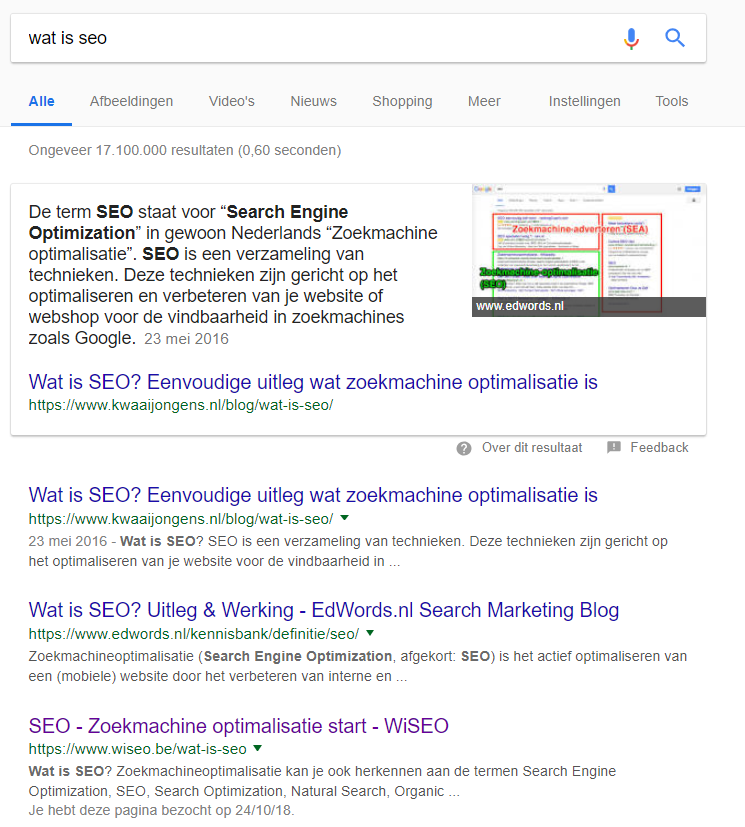
\includegraphics[width=\linewidth]{img/watisseo.png}
\caption{Een afbeelding die een screenshot van de zoekresultaten in Google voor het zoekwoord 'wat is seo' \autocite{google.be}}
\end{figure}

Er zijn bestaan meerdere zoekmachines zoals Bing en Yahoo! maar de meest gebruikte is Google. In dit onderzoek wordt dan ook uitsluitend gewerkt met Google omdat ze meer dan 92\% van het marktaandeel in handen hebben en de focus van WiSEO ook bij Google ligt. Bing en Yahoo! hebben maar elk iets meer dan 5\% marktaandeel samen (op 10/12/2018),          
\textcite{ZOEKMACHINES} .

SEO gaat altijd gepaard met het gebruik van allerlei tools. Deze tools helpen sterk bij: 
\begin{itemize}
\item Het vinden van de juiste zoekwoorden waarop een website moet scoren.
\item Het bekijken van de concurrentie in dezelfde sector of niche.
\item Het controleren alle technische SEO-aspecten op een website.
\item Het vinden van potentiële backlinks (een verwijzing van een andere webpagina naar de eigen site door middel van een link) en zo hoger in de zoekmachine resultaten te komen door autoriteit op te bouwen. Hoe meer inkomende links naar je eigen website, hoe meer dat Google je website als ‘belangrijk’ aanziet. 
\end{itemize}

Kortom, het is bijna onmogelijk om een website te optimaliseren zonder tools te gebruiken voor deze verschillende aspecten.

Op dit moment is er nog geen compleet onderzoek gedaan naar een vergelijking tussen SEO-tools en het resultaat dat ze opleveren. De reden dat dit moet worden onderzocht is omdat WiSEO hierdoor de opdrachten voor middelgrote bedrijven beter kan uitvoeren door middel van een beter zoekwoordenonderzoek, beter concurrentieonderzoek… met als eindresultaat een hogere score in de zoekresultaten.

Het onderzoek bestaat uit 2 delen. Aan de ene kant bestaat het uit een literatuurstudie waar verschillende tools met elkaar vergeleken worden door verschillende aspecten zoals prijs, soort tool en welke gegevens ze opleveren (en dus welke functionaliteiten ze bevatten). Anderzijds wordt een technische uitwerking voorzien door het verbeteren van een SEO-keyword tool. De tool wordt helemaal van nul geprogrammeerd maar een deel van de werking blijft hetzelfde als een tool die al bestaat. 


\section{Stand van zaken in het onderzoeksdomein}
\label{sec:Stand van zaken in het onderzoeksdomein}

In dit onderzoeksdomein zijn er al dergelijke onderzoeken uitgevoerd die vaak in de vorm van blogartikelen terug te vinden zijn. Veel van deze artikelen bijvoorbeeld geven de beste SEO-tools \textcite{SEO13} weer of een volledige lijst van SEO-tools in 2018 \textcite{SEOCOMPLETE}. Ze hebben relevantie tot het onderzoek dat hier gevoerd wordt in de zin dat er ook een vergelijking zal gebeuren tussen meerdere SEO-tools. 

Bij vele van deze blog artikelen wordt er wel geen duidelijk onderscheid gemaakt welke informatie je precies verkrijgt bij een bepaalde tool. Er worden veel tools vermeld waar er tijdelijke trials voor zijn maar je dan achteraf maandelijks een bedrag moet neerleggen. De eerste onderzoeksvraag zal duidelijk het verschil maken tussen gratis en betaalde tools. 


\section{Probleemstelling}
\label{sec:probleemstelling}

Vele SEO-tools in deze vermelde blogartikelen zijn tamelijk duur geprijsd (in de literatuurstudie zal duidelijk zijn wat duur is en wat niet) terwijl er betere alternatieven op de markt bestaan. De meeste tools zijn trials die na verloop van tijd betalend zijn en duur kunnen worden, dit wordt vaak niet of weinig vermeld. Andere tools bieden dan een gratis versie aan maar daar staan altijd beperkingen op. 

Bij de literatuurstudie wordt ook aangetoond dat WiSEO veel tijd verliest met zoekwoordonderzoeken doordat ze handmatig keywords in zoekwoordgroepen moet plaatsen met een Spreadsheet. Daarbij zal er gesuggereerd worden waarom er zelf een keyword tool wordt uitgewerkt. Dit zal gebeuren door een bestaande zoekwoord tool te verbeteren. 


\section{Onderzoeksvragen}
\label{sec:onderzoeksvragen}

Dit onderzoek bestaat uit 2 grote delen waar dan ook meteen 2 onderzoeksvragen uit voorkomen. 

De eerste onderzoeksvraag luidt als volgt: “Welke SEO-tools kunnen best als hulpmiddel gebruikt worden voor meer zichtbaarheid in zoekmachines?”. Hierbij zal een vergelijkende studie gebeuren tussen 4 verschillende soorten tools namelijk: 

\begin{itemize}
\item Zoekwoord onderzoek tools: deze tools worden gebruikt om op zoek te gaan naar de juiste zoekwoorden die je moet gebruiken in je SEO-campagne. Daarbij is het de bedoeling om te zorgen voor betere content (met de juiste zoekwoorden) om het bezoek naar de website op belangrijke zoekwoorden vanuit Google te verhogen. 
\item Ranking tools: hierbij kun je makkelijk zien op welke positie bepaalde zoekwoorden staan in Google voor jouw website. Op die manier kun je snel zien welke zoekwoorden hoog scoren en waar niet. 
\item Backlink tools: backlinks gaan over de autoriteit van een website. Hoe meer links een website heeft van andere websites, hoe meer autoriteit en dus een betere score in Google. Met deze tools kun je bekijken hoeveel links een bepaalde website heeft van andere domeinen en ook welke deze precies zijn. Daarnaast geven sommige tools ook een indicatiescore van de waarde van een domein, hoe meer waarde hoe meer autoriteit in Google.
\item Technische tools: deze tools controleren de technische kant van een website. Hierbij wordt onder andere gekeken naar de metagegevens, de hiërarchie van de URL-structuur en de sitemap van een site.  
\end{itemize}

Aan de hand van enkele aspecten wordt er dan uitgemaakt welke tool de duidelijkste informatie oplevert die SEO'ers (WiSEO en andere SEO-bureaus) het best kunnen gebruiken. Deze aspecten zullen allemaal duidelijk worden uitgelegd in de inleiding van de literatuurstudie. Voor elke soort zal ook een prijsvergelijking plaatsvinden. 

De tweede onderzoeksvraag is: “Hoe gebeurt het verbeteren van een keyword tool zodat er vlotter een zoekwoordonderzoek uitgevoerd kan worden?”. Hierbij zal een eigen tool geprogrammeerd worden om aan te tonen dat er nog verbetering mogelijk is bij zoekwoord tools. 

Er zal een keyword tool geprogrammeerd worden in Java met een eigen ontwerp door gebruik te maken van JavaFX Scene Builder. 


\section{Doelstellingen}
\label{sec:doelstellingen}

% Het is gebruikelijk aan het einde van de inleiding een overzicht te
% geven van de opbouw van de rest van de tekst. Deze sectie bevat al een aanzet
% die je kan aanvullen/aanpassen in functie van je eigen tekst.

De rest van deze bachelorproef is als volgt opgebouwd:

In Hoofdstuk~\ref{ch:studie} wordt er een oplijsting  weergegeven van verscheidene tools. Daarbij zal het duidelijk zijn welke tools best gebruikt kunnen worden per soort tool (zoekwoordonderzoek tools, ranking tools, backlink tools en technische tools) waarbij rekening gehouden wordt met de prijs ervan. De doelstelling is uiteindelijk ook om aan te tonen dat dure tools niet altijd de beste tools zijn en er betere (en goedkopere) alternatieven zijn. 

In Hoofdstuk~\ref{ch:tool} wordt de methodologie toegelicht en worden de gebruikte onderzoekstechnieken besproken om een antwoord te kunnen formuleren op de onderzoeksvragen.

% TODO: Vul hier aan voor je eigen hoofstukken, één of twee zinnen per hoofdstuk

In Hoofdstuk~\ref{ch:conclusie}, tenslotte, wordt de conclusie gegeven en een antwoord geformuleerd op de onderzoeksvragen. 


\chapter{Vergelijkende studie tussen SEO-tools}
\label{ch:Vergelijkende studie tussen SEO-tools}

In deze literatuurstudie zal er een vergelijking gemaakt worden tussen verschillende SEO-tools. Hierbij worden de SEO-tools in 4 grote categorieën opgedeeld, namelijk: zoekwoord onderzoek tools, ranking tools, backlink tools en technische tools. De geteste tools komen uit enkele populaire artikels, \textcite{SEOCOMPLETE} en \textcite{SEO13}, maar ook uit de tools waar WiSEO al gebruikt van maakt. 

Per soort SEO-tool wordt een beoordeling gegeven aan de hand van een aantal aspecten. Deze geteste aspecten worden per soort tool duidelijk aangegeven. 

Het komt wel voor dat tools meerdere doeleinden hebben (bijvoorbeeld: een zoekwoord en ranking tool in één of zogeheten ‘all-in-one tools’). Deze tools worden dan beoordeeld per aspect. Het zal voorkomen dat dezelfde tool meerdere keren gebruikt wordt in verschillende categorieën. 

Na elk onderzoek zal per onderdeel een tabel gemaakt worden met alle tools en de aspecten ervan om een duidelijk overzicht te krijgen van welke tool het best gebruikt kan worden (prijs/kwaliteit). 

\section{Zoekwoorden onderzoek tools}
\label{ch: Zoekwoorden onderzoek tools}

\subsection{Doel van een zoekwoordenonderzoek}
\label{ch: Doel van een zoekwoorden onderzoek}

Een zoekwoordonderzoek is onmisbaar bij elke SEO-campagne. Voordat er van start gegaan wordt met zoekmachineoptimalisatie op een website, moet eerst duidelijk zijn op welke zoekwoorden een bepaalde site wil scoren. Zelfs bij adverteren is het nodig om te weten welke zoekwoorden potentiële websitebezoekers gebruiken. 

Met zo’n onderzoek krijgt men inzicht in de woordkeuze van een bepaalde doelgroep. Op die manier komen vaak zoekwoorden naar boven waar men anders niet aan gedacht zou hebben. Keyword research is praktisch onmogelijk uit te voeren zonder gebruik te maken van tools, waarbij je onder andere zoekwoordsuggesties en het gemiddelde maandelijks zoekvolume te zien krijgt. 

Het is ten slotte ook belangrijk om inzicht te krijgen in de de zoekwoorden gebruikt door de concurrentie waarop er ingespeeld moet worden. Het is belangrijk om te controleren of er een analyse gemaakt is van de competitie of de moeilijkheidsgraad om te scoren op een bepaald zoekwoord. Met de competitie of moeilijkheidsgraad wordt er een indicatie, meestal een score (verschilt per tool), meegegeven hoe moeilijk het is om boven andere websites (concurrenten) te staan voor een bepaald zoekwoord (op de eerste positie in Google). 

\subsection{Geteste aspecten}
\label{ch: Geteste aspecten}

De vergelijkende studie tussen keyword tools gebeurt aan de hand van een aantal geteste aspecten. Hierbij bekijkt men wat belangrijk is om een zoekwoordonderzoek uit te voeren. Alle onderdelen staan hieronder opgesomd: 

\begin{itemize}
\item Prijs: er zal gekeken worden of er een gratis versie of tijdelijke trial bestaat en wat de (maandelijkse) kostprijs is van de tool. Sommige tools hebben beperkingen bij de gratis versie of trial en dit zal duidelijk gemaakt worden in het onderzoek. 
\item Zoekvolume per maand: geeft het gemiddelde zoekvolume weer per maand voor een zoekwoord. Dit is het aantal keer dat een zoekwoord in de Google zoekbox ingegeven wordt per maand.
\item Aantal zoekwoorden per dag: het aantal zoekwoorden dat je dagelijks kan opzoeken. Bij gratis versies of trials wordt dit vaak beperkt zodat je sneller de betaalde versie zou kopen. Met ‘opzoeken’ wordt bedoeld dat je een zoekwoord ingeeft en hiervoor gerelateerde zoekwoorden krijgt.
\item Suggesties van gerelateerde zoekwoorden: het is interessant om bij het ingeven van een keyword suggesties te krijgen van gerelateerde zoekwoorden. Bijvoorbeeld voor het zoekwoord: ‘restaurant Brugge’ krijg je dan verwante zoekwoorden te zien zoals: ‘bistro Brugge’ en ‘eten in Brugge’.
\item Pay per click: geeft een bedrag aan wat de gemiddelde kost per klik is voor een advertentie in Google. Een advertentie (Adv.) ziet er zo uit en de prijs per persoon die op zo’n link klikt is de pay per click of PPC: 

\begin{figure}[h!]
\centering
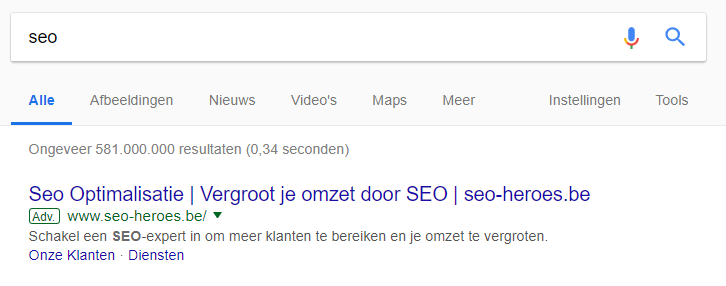
\includegraphics[width=\linewidth]{Bachelorproef/bachelor/img/Adwordsvoorbeeld.png}
\caption{Een afbeelding die een screenshot van de zoekresultaten in Google voor het zoekwoord 'seo', de eerste advertentie wordt getoond \autocite{google.be}}
\end{figure}

\item Moeilijkheid om te scoren en analyse van de concurrentie: het is belangrijk om te weten of het mogelijk is om te concurreren op een bepaald zoekwoord. Geeft de keyword tool een bepaalde indicatie van moeilijkheidsgraad om bovenaan te staan bij een bepaald zoekwoord? 
\item Locatie en taal: hoe specifiek kan je een bepaalde locatie ingeven (de personen die vanuit bepaalde locaties zoeken op bepaalde keywords, dit kan een land of, nog specifieker, een stad zijn) en de taal waarin het zoekwoord gezocht wordt. 
\item SERP analyse: SERP betekent simpelweg de resultatenpagina van een zoekmachine, wat je dus te zien krijgt wanneer je een zoekopdracht hebt ingevoerd in Google. Het is interessant om een duidelijk overzicht te krijgen om te weten welke websites de eerste tien plaatsen innemen en zo meer informatie te verkrijgen over deze concurrenten. 
\end{itemize}

\subsection{Vergelijkende studie tussen keyword tools}
\label{ch: Vergelijkende studie tussen keyword tools}

De keyword tools die getest worden zijn: Zoekwoordplanner, Ubersuggest, Keywordtool.io, KwFinder en Moz. De reden dat deze 5 tools werden uitgekozen is omdat Zoekwoordplanner en Ubersuggest worden gebruikt bij WiSEO en ze worden vermeld in deze artikels: \textcite{SEO13} en \textcite{SEOCOMPLETE}. 

\subsubsection{Zoekwoordplanner}
\label{ch: Zoekwoordplanner}
Er bestaan twee versies van de zoekwoordplanner. Wanneer je geen actief Adwordsbudget uitgeeft dan krijg je slechts een ruime schatting te zien van het gemiddeld maandelijks zoekvolume (bv: tussen de 10 en 100 of tussen de 100 en 1000). Dit ziet er als volgt uit:  

\begin{figure}[h!]
\centering
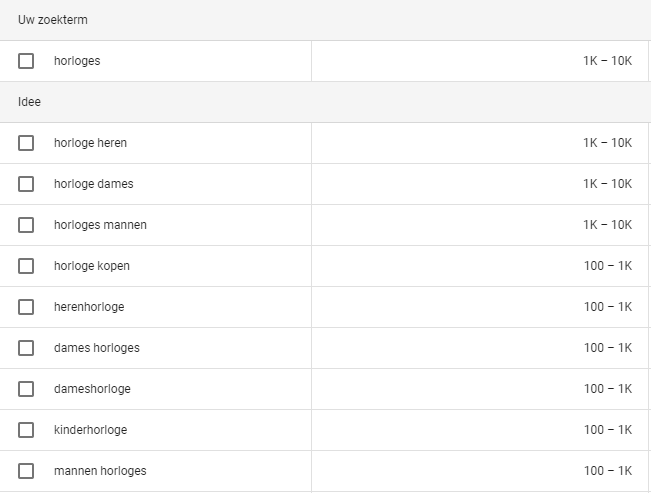
\includegraphics[width=\linewidth]{Bachelorproef/bachelor/img/Zoekwoordplannergratis.PNG}
\caption{Een screenshot van de zoekwoordplanner zonder actief Adwordsbudget \autocite{google.be}}
\end{figure}

Indien er een Adwordsbudget uitgegeven wordt (de exacte cijfers van dit budget zijn niet vrijgegeven door Google) dan krijg je wel het exacte maandelijks zoekvolume te zien: 

\begin{figure}[h!]
\centering
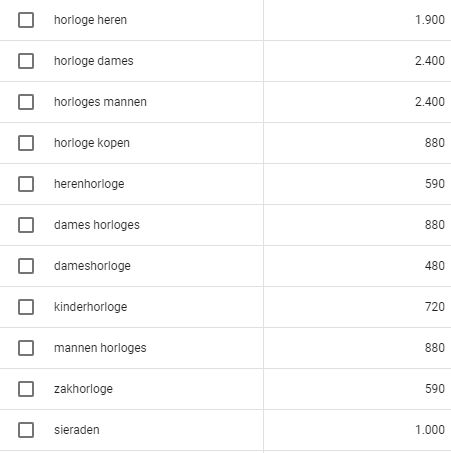
\includegraphics[width=\linewidth]{Bachelorproef/bachelor/img/Zoekwoordplannerbet.PNG}
\caption{Een screenshot van de zoekwoordplanner met actief Adwordsbudget \autocite{google.be}}
\end{figure}

Je krijgt een ongelimiteerd aantal query's van zoekwoorden die je kan opzoeken. Daarnaast krijg je ook telkens suggesties van gerelateerde zoekwoorden. 

De PPC (Pay per Click) wordt aangegeven. Er is een kolom die aangeeft wat de concurrentie is (laag-normaal-hoog). Dit betreft de concurrentie voor advertenties op Google, niet de organische (SEO) concurrentie. Naast de tabel van de concurrentie staat het gemiddelde bod (per klik naar je website) om bovenaan de pagina te komen in Google met een advertentie (hoog bereik). In de rechtertabel staat het gemiddeld bod om bovenaan de pagina te komen met een advertentie (laag bereik). 

\begin{figure}[h!]
\centering
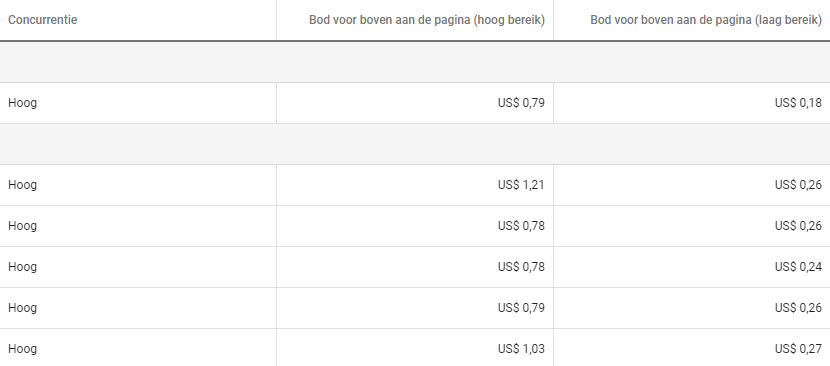
\includegraphics[width=\linewidth]{Bachelorproef/bachelor/img/Zoekwoordplannercon.PNG}
\caption{Een screenshot van de rechterkolommen van de zoekwoordplanner met de concurrentie en gemiddelde Adwordsprijs per klik \autocite{google.be}}
\end{figure}

Ten slotte kan je de locatie (op stedelijk niveau) en de gewenste taal instellen. Er is geen SERP analyse van de tool.

\subsubsection{Ubersuggest}
\label{ch: Ubersuggest}

Ubersuggest is een tool die gratis te gebruiken is. Er worden zoekwoordsuggesties getoond samen met het maandelijks gemiddeld zoekvolume. Dagelijks kan je een ongelimiteerd aantal zoekwoorden opzoeken. De gemiddelde PPC (Pay per Click) wordt aangegeven. SD geeft een score die aangeeft wat de competitie is in Google voor dat zoekwoord. 

\begin{figure}[h!]
\centering
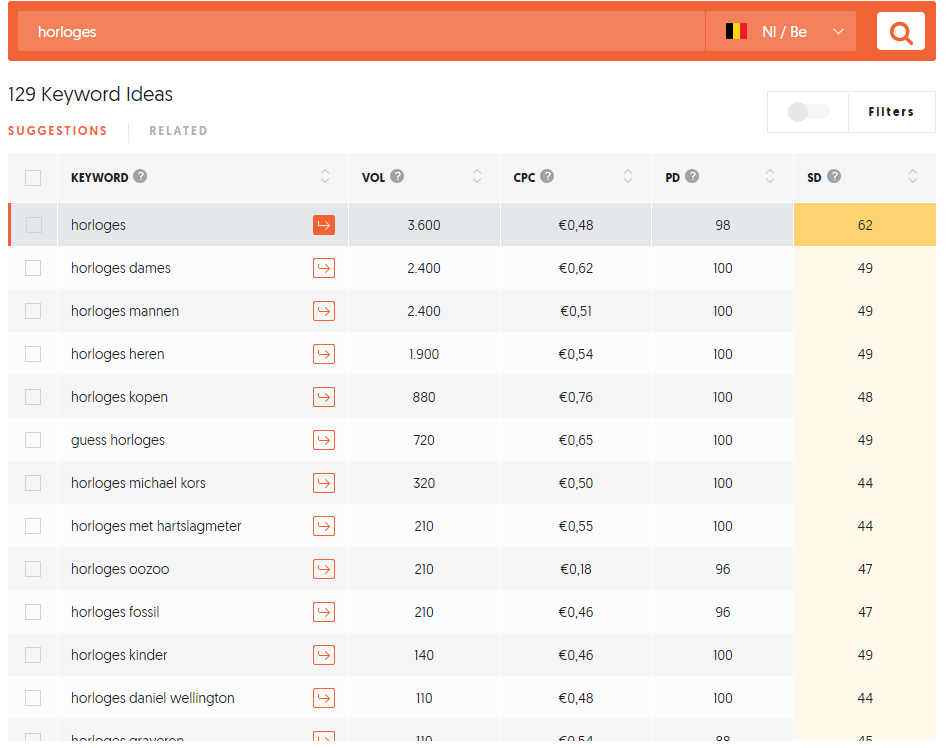
\includegraphics[width=\linewidth]{Bachelorproef/bachelor/img/ubers.PNG}
\caption{Een screenshot van de Ubersuggest tool, zoekwoordsuggesties \autocite{ubersuggest}}
\end{figure}

In de rechterkolom zie je de top-zoekresultaten (voor dat bepaald zoekwoord) waarbij een link, het gemiddeld aantal bezoekers en de domeinscore te zien is. Met de domeinscore wordt het volgende bedoeld: op basis van verschillende factoren (deze factoren zijn niet vrijgegeven door Ubersuggest) is dit de algemene sterkte van de website. Een score van 1 tot 100 wordt gegeven aan alle websites, hoe hoger het cijfer, hoe meer autoriteit een website heeft en hoe hoger de positie van een website kan zijn op Google. 

Ten slotte kan je de locatie (op landelijk niveau) en de gewenste taal instellen. 

\begin{figure}[h!]
\centering
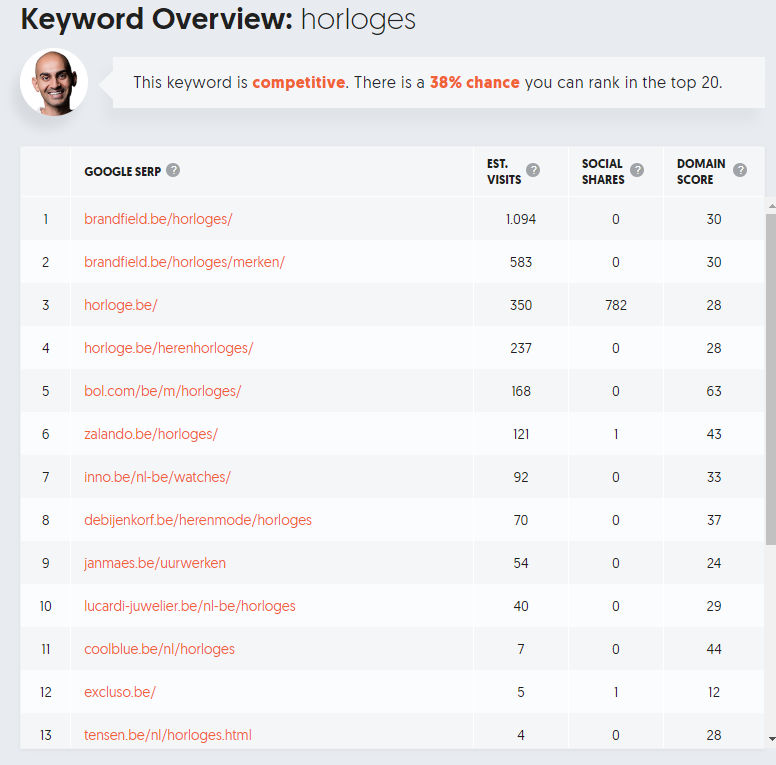
\includegraphics[width=\linewidth]{Bachelorproef/bachelor/img/ubersrechts.PNG}
\caption{Een screenshot van de Ubersuggest tool, de Google SERP \autocite{ubersuggest}}
\end{figure}

\subsubsection{Keywordtool.io}
\label{ch: Keywordtool.io}

Bij de gratis versie krijg je enkel de zoekwoordsuggesties te zien. Je ziet geen zoekwoordvolume, CPC (of PPC) en competitie van het zoekwoord. 

Je kan een ongelimiteerd aantal zoekwoorden opzoeken, zowel betalend als gratis. 

De betalende versie waarbij je zoekwoordsuggesties met het maandelijks zoekvolume te zien krijgt, kost 88 dollar per maand. De gemiddelde PPC (Pay per Click) wordt uitgedrukt in Amerikaanse dollars. Helemaal rechts is de competitie te zien voor Google Adwords (niet voor organische zoekresultaten). 

\begin{figure}[h!]
\centering
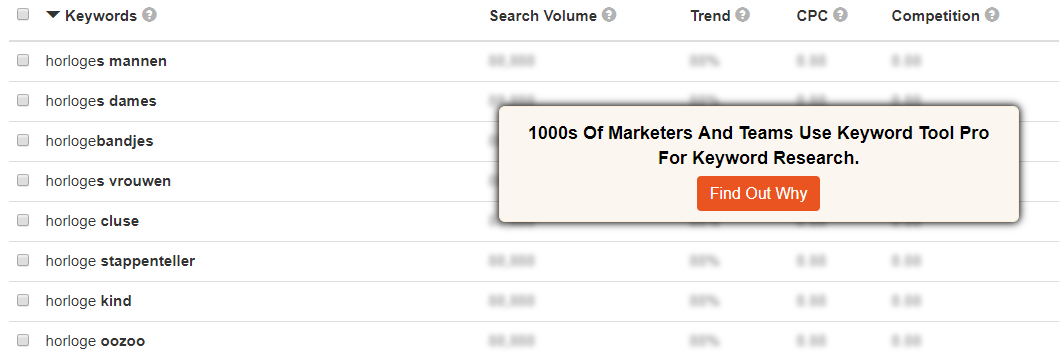
\includegraphics[width=\linewidth]{Bachelorproef/bachelor/img/keywordtoolio.PNG}
\caption{Een screenshot van de zoekwoordsuggesties van Keywordtool.io \autocite{keywordtoolio}}
\end{figure}

Ten slotte kan je de locatie (op landelijk niveau) en de gewenste taal instellen.

\subsubsection{KwFinder}
\label{ch: KwFinder}

Er is een gratis versie waarbij er 5 zoekwoorden per dag kunnen opgezocht worden. Per zoekwoord worden tot 25 zoekwoordsuggesties gegeven. 

Er zijn 3 betalende versies: 

\begin{itemize}
\item 25,90 euro per maand - 100 zoekwoorden per dag - 200 suggesties per zoekwoord.
\item 34,90 euro per maand - 500 zoekwoorden per dag - 700 suggesties per zoekwoord.
\item 69,90 euro per maand - 1200 zoekwoorden per dag - 700 suggesties per zoekwoord.
\end{itemize}

Per zoekwoord wordt de gemiddelde Cost per Click weergeven voor Google Adwords. Daarnaast zie je ook de competitie voor een zoekwoord (Google Adwords). 

Er is een duidelijke moeilijkheidsgraad door de KD (Keyword SEO difficulty): hoe hoger de score, hoe moeilijker om hoog te ranken met dit zoekwoord. 

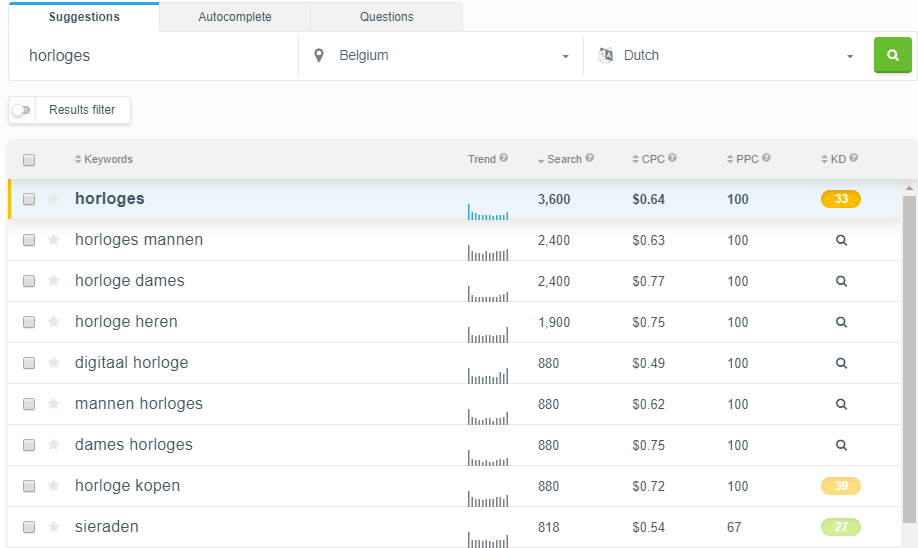
\includegraphics[width=\linewidth]{Bachelorproef/bachelor/img/kwfinderlinks.PNG}
(Een screenshot van de zoekwoordsuggesties van Kwfinder, linkerkant)

In de rechterkolom zie je de eerste tien websites te zien die te vinden zijn in Google. DA, PA, CF en TF zijn waardes die de domein- en paginawaarde van een bepaalde website uitdrukken. LPS is een combinatie van die 4 waardes en geeft de algemene link sterkte (overall Link Profile Strength) weer. 

EV laat zien hoeveel bezoekers deze website gemiddeld per maand krijgt voor een bepaald zoekwoord. 

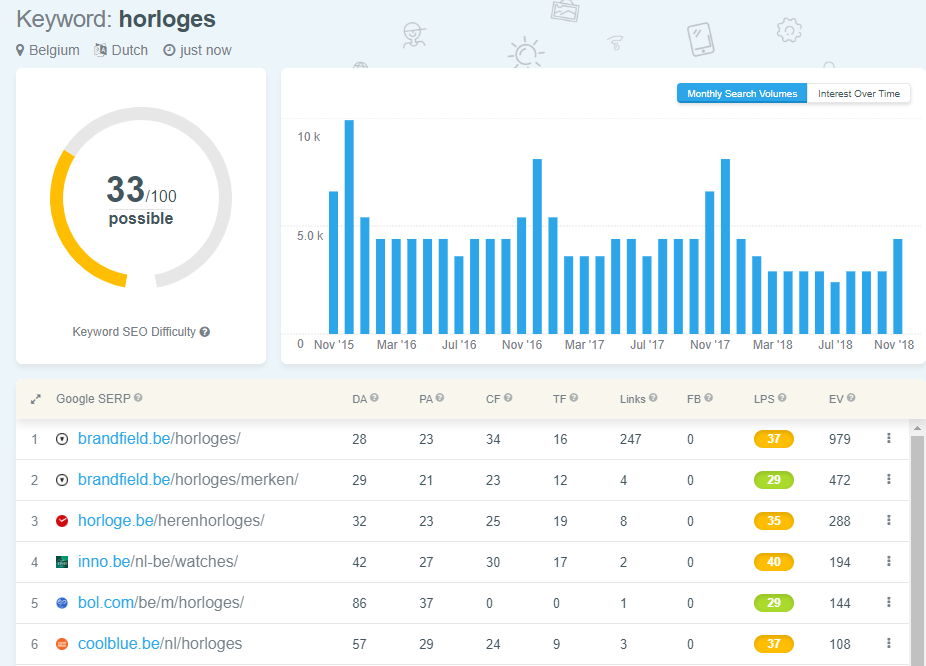
\includegraphics[width=\linewidth]{Bachelorproef/bachelor/img/kwfinderrechts.PNG}
(Een screenshot van de Google SERP van Kwfinder, rechterkant)

Ten slotte kan je de locatie (op landelijk niveau) en de gewenste taal instellen.

\subsubsection{Moz}
\label{ch: Moz}

Bij de gratis versie kan je tot 10 keywords opzoeken per maand. Voor elk zoekwoord krijg je zoekwoordsuggesties.

Er zijn 3 betalende versies 

\begin{itemize}
\item 99 dollar per maand - 150 zoekwoorden per maand - 10000 suggesties per zoekwoord.
\item 179 dollar per maand - 5000 zoekwoorden per maand - 30000 suggesties per zoekwoord.
\item 249 dollar per maand - 15000 zoekwoorden per maand - 50000 suggesties per zoekwoord.
\item 999 dollar per maand - 30000 zoekwoorden per maand - 100000 suggesties per zoekwoord.
\end{itemize}

De gemiddelde advertentieprijs (PPC) is niet te zien. Je kan een difficulty score (concurrentie) zien tussen 0 en 100 voor een bepaald zoekwoord. Deze score geeft aan hoe moeilijk het is om hoog te ranken voor dit zoekwoord. 

Voor België krijg je geen zoekwoordvolume te zien. (Noch gratis, noch betalend.)

Je krijgt een duidelijk overzicht van de eerste negen zoekresultaten in Google voor een bepaald zoekwoord. 

Ten slotte kan je de locatie (op landelijk niveau) en de gewenste taal instellen.

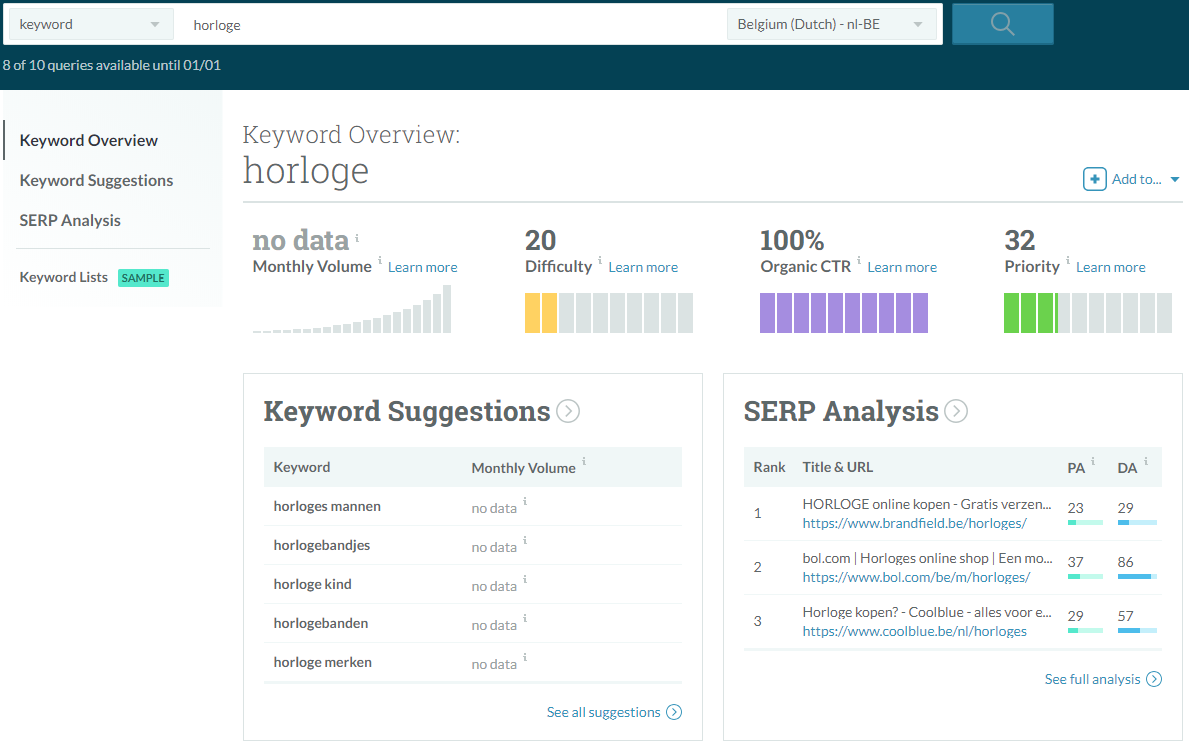
\includegraphics[width=\linewidth]{Bachelorproef/bachelor/img/moz.PNG}
(Een screenshot van de zoekwoordsuggesties van Moz)

\subsection{Overzicht}
\label{ch: Overzicht}

In de volgende tabel wordt een overzicht gegeven van alle besproken tools. 

Korte legende: 
\begin{itemize}
\item Rood: niet aanwezig in de tool
\item Groen: wel aanwezig in de tool
\end{itemize}

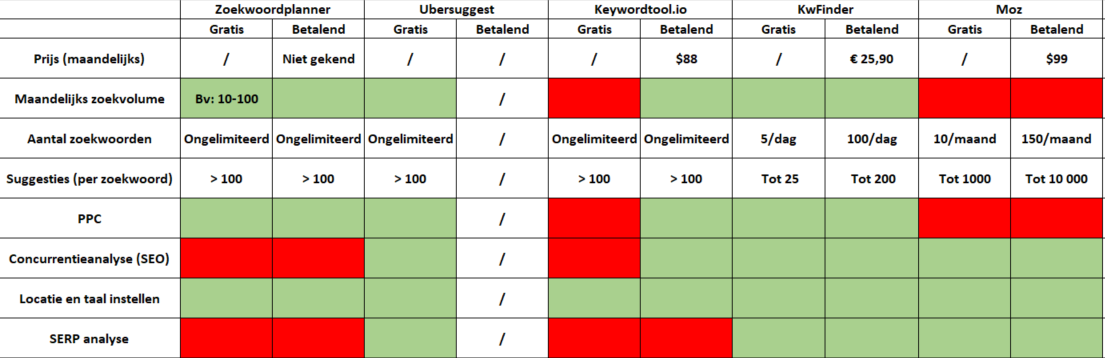
\includegraphics[width=\linewidth]{Bachelorproef/bachelor/img/zoekwoordtabel.PNG}
(Tabel met een duidelijk overzicht van alle functionaliteiten van de zoekwoord tools)

Extra opmerking bij de tabel (locatie en taal instellen): Het is enkel bij de zoekwoordplanner mogelijk om de locatie in te stellen op stedelijk niveau. Alle andere tools kan je instellen op landelijk niveau. 

In het besluit zullen de beste gratis en betalende tool gekozen worden.

De beste gratis tool is Ubersuggest. Met de tool KwFinder (die ook aan alle criteria voldoet) kan je slechts vijf zoekwoorden per dag opzoeken, terwijl je met Ubersuggest ongelimiteerd kunt opzoeken. Daarbij geeft Ubersuggest meer dan honderd zoekwoordsuggesties, bij KwFinder zijn dit er slechts vijfentwintig. 
De beste betalende tool is KwFinder. Vanaf 25,90 euro per maand kan je al 100 zoekwoorden per dag opzoeken en telkens 200 zoekwoordsuggesties krijgen. Verder voldoet de tool ook aan alle opgesomde criteria. 

\section{Ranking tools}
\label{ch: Ranking tools}

\subsection{Doel van een ranking tool}
\label{ch: Doel van een ranking tool}

Het is belangrijk om te weten welke positie je in Google bekleedt voor keywords die relevant zijn voor je website. Deze tools worden gebruikt om de positie van een website voor bepaalde zoekwoorden te controleren. 

Bij zo’n onderzoek kom je snel te weten voor welke zoekwoorden je net niet op de eerste plek of binnen de top 10 staat, en hierop kan je dan specifiek inspelen.

Het is niet aan te raden om je enkel te baseren op de resultaten vanop je eigen laptop die je in Google te zien krijgt. Je eigen resultaten worden beïnvloed door de huidige locatie en vorige zoekopdrachten. Het is ten slotte ook veel werk om tientallen zoekwoorden handmatig in te typen. 

\subsection{Geteste aspecten}
\label{ch: Geteste aspecten}

De vergelijkende studie tussen ranking tools gebeurt met een aantal geteste aspecten. Hierbij wordt gekeken naar wat belangrijk is om een rankingonderzoek uit te voeren. Alle onderdelen staan hieronder opgesomd: 

\begin{itemize}
\item Prijs: er zal gekeken worden of er een gratis versie of een tijdelijke trial is en wat de kostprijs van de tool is (maandelijks). Sommige tools hebben beperkingen bij de gratis versie of trial en dit zal duidelijk gemaakt worden in het onderzoek. 
\item Difficulty scoring: geeft de moeilijkheid aan om voor een bepaald zoekwoord op de eerste positie te komen in Google.
\item Competitor analysis: het is handig om meer te weten te komen over de websites die ook hoog ranken voor een bepaald zoekwoord. Op die manier kan je inschatten wie de concurrentie is en hoe moeilijk het is om op een hogere positie te komen voor een keyword.
\item Aantal keywords: hoeveel keywords kan je tegelijk tracken? 
\item Aantal domeinen: hoeveel domeinen kan je tegelijk tracken? 
\item Dagelijke, wekelijkse of maandelijkse ranking check: hoeveel keer worden de rankings per dag/week/maand bekeken. 
\item Indicatie van verandering: geeft de tool een indicatie mee of er verandering is in de ranking in vergelijking met gisteren, vorige week of vorige maand?
\item Locatie en taal: hoe specifiek kan je een bepaalde locatie ingeven (de personen die vanuit bepaalde locaties zoeken op bepaalde keywords, dit kan een land of, nog specifieker, een stad zijn) en de taal waarin het zoekwoord gezocht wordt.  
\end{itemize}

\subsection{Vergelijkende studie tussen ranking tools}
\label{ch: Vergelijkende studie tussen ranking tools}

De tools die worden onderzocht zijn Semrush, Rank tracker, AWR Cloud en Accuranker. De reden dat deze 4 tools werden uitgekozen is omdat AWR Cloud wordt gebruikt bij WiSEO en ze worden vermeld in deze artikels: \textcite{SEO13} en \textcite{SEOCOMPLETE}.  

\subsubsection{Semrush}
\label{ch: Semrush}
De tool Semrush heeft een gratis versie waarbij er 1 website getrackt kan worden tot maximum tien zoekwoorden. Dit betekent dat je met de software voor 1 domein tegelijk 10 zoekwoorden kan opvolgen (kijken op welke positie ze staan en bekijken als je website gestegen of gedaald is van positie). 

Bij de kolom 'diff' zien we de positieverandering in vergelijking met 7 dagen geleden. Deze tijdsperiode kan je instellen voor 2 dagen, een week, een maand, 2 maanden en 3 maanden. 

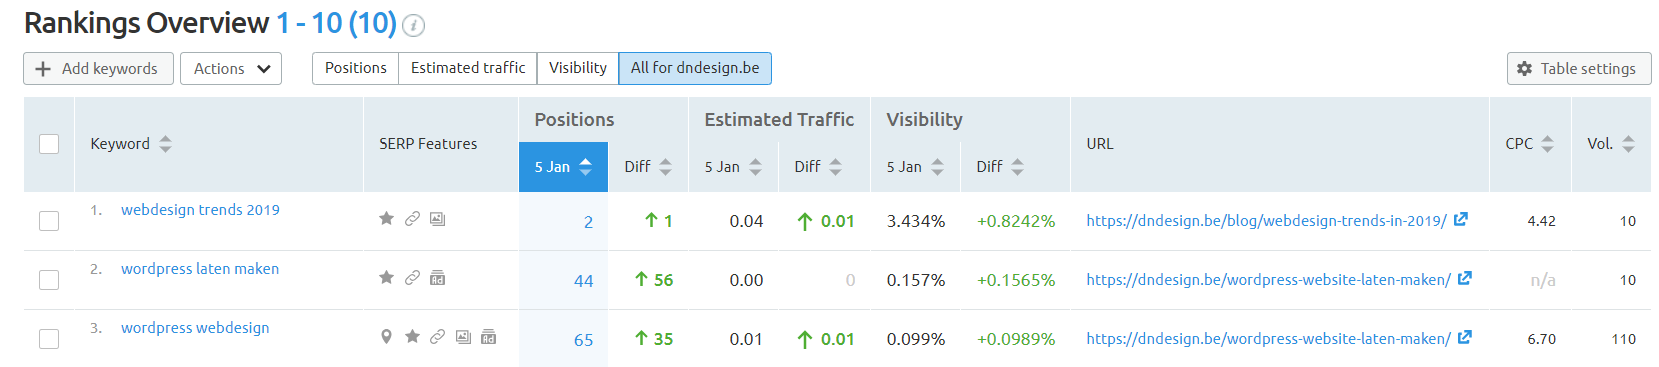
\includegraphics[width=\linewidth]{Bachelorproef/bachelor/img/semrushranking.PNG}
(Screenshot van de werking van de Semrush tool voor de zoekwoorden)

De betalende versies: 
\begin{itemize}
\item 99,95 dollar per maand - tot 5 websites - tot 500 keywords
\item 199,95 dollar per maand - tot 50 websites - tot 1500 keywords
\item 399,95 dollar per maand - tot 200 websites - tot 5000 keywords
\end{itemize}

Bij het aanmaken van een project heb je de mogelijkheid om zoekwoorden in te vullen die je wil tracken. 

Het is mogelijk om je eigen concurrenten in te geven in de tool. Zo kan je zien op welke positie zij staan voor bepaalde zoekwoorden. Voorbeeld van de positie van een zoekwoord van een concurrent: 

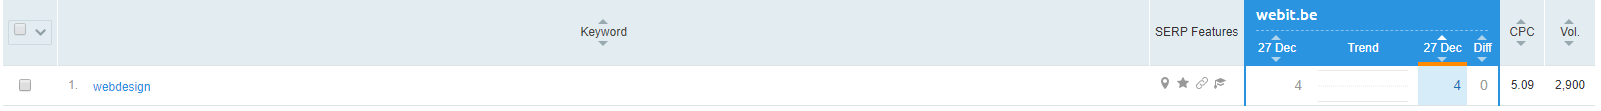
\includegraphics[width=\linewidth]{Bachelorproef/bachelor/img/semrushcompetitie.PNG}

(Screenshot van de werking van de Semrush tool voor de competitie)

De tool geeft een indicatie van verandering mee (het aantal posities dat je website verschoven is in Google). Je kan het verschil zien per dag. 

Bij de tool kan je zelf de taal en het land instellen. 

\subsubsection{AWR Cloud}
\label{ch: AWR Cloud}
Bij AWR Cloud kan je voor 30 dagen een trial aanmaken. Hierbij moet je wel een kredietkaart ingeven. Na deze 30 dagen wordt 49 dollar aangerekend. 

De betalende versies: 
\begin{itemize}
\item 49 dollar per maand - tot 2000 keywords
\item 99 dollar per maand - tot 7000 keywords
\item 199 dollar per maand - tot 14500 keywords
\end{itemize}

Bij het aanmaken van een project is het mogelijk om zoekwoorden in te vullen die je wil tracken. Je kan de huidige positie zien van deze zoekwoorden en de wekelijkse verandering. 

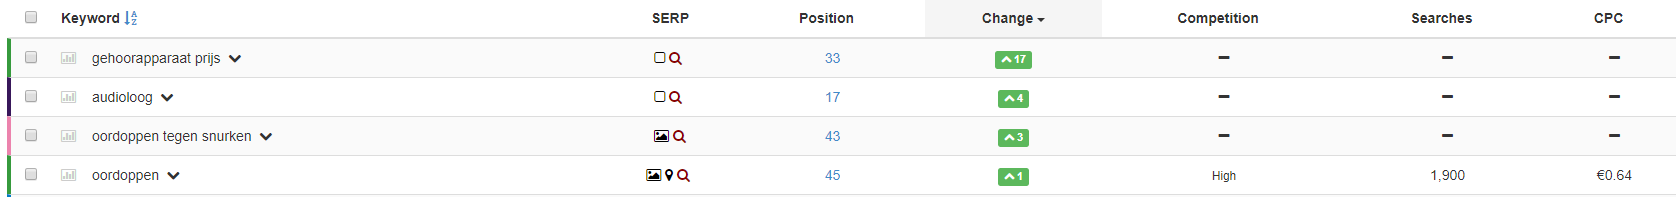
\includegraphics[width=\linewidth]{Bachelorproef/bachelor/img/awrcloud.PNG}
(Werking van de AWR cloud tool voor verschillende zoekwoorden)

De visibility score of visibiliteitsscore is een handige metric om een totaaloverzicht te verkrijgen van de evolutie van alle zoekwoorden. De score wordt berekend door een formule gebaseerd op wekelijkse zoekwoordrankings. Het geeft een inzicht in de evolutie voor alle zoekwoorden. 

Om de visibility score te berekenen worden er punten toegekend als volgt :
\begin{itemize}
\item Positie 1 (pagina 1 in Google, de eerste SEO positie) : 30 punten
\item Positie 2 (pagina 1 in Google, de tweede SEO positie) : 29 punten
\item …
\item Positie 30 (pagina 3 in Google, de tiende SEO positie) : 1 punten
\end{itemize}
Posities onder 30 krijgen geen punten.

De visibility score is de som van de punten die per zoekwoord zijn toegekend.

Met deze score kan je wekelijks checken of er vooruitgang is geboekt en vergelijken met je concurrenten. Dit ziet er als volgt uit: 

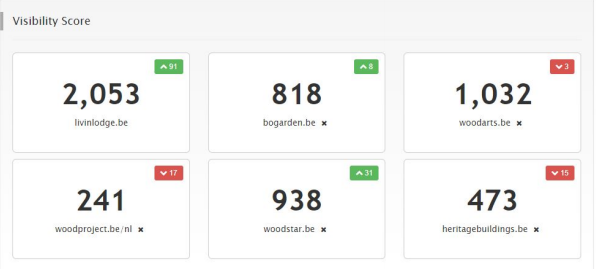
\includegraphics[width=\linewidth]{Bachelorproef/bachelor/img/awrcloudvisibility.PNG}
(Visibility score tussen verschillende websites)

Het is dus mogelijk om met de tool je eigen concurrenten in te geven.

De competitie voor een bepaald zoekwoord wordt aangegeven door de termen high-medium-low. 

Bij de tool kan je zelf de taal en het land instellen. 

\subsubsection{Rank Tracker}
\label{ch: Rank Tracker}

De gratis versie laat toe om tot 2 websites te koppelen en 20 zoekwoorden in totaal in te vullen. Deze trial duurt 10 dagen. 

De betalende versies: 
\begin{itemize}
\item 22 euro per maand - tot 3 domeinen - tot 250 keywords
\item 68 euro per maand - tot 10 domeinen - tot 1000 keywords
\item 128 euro per maand - ongelimiteerd aantal domeinen - tot 1750 keywords
\end{itemize}

Je krijgt een duidelijk overzicht met de zoekwoorden die je gekozen hebt. Per dag/week/maand kan je de ranking zien in Google en ook vergelijken met een vorige periode. 

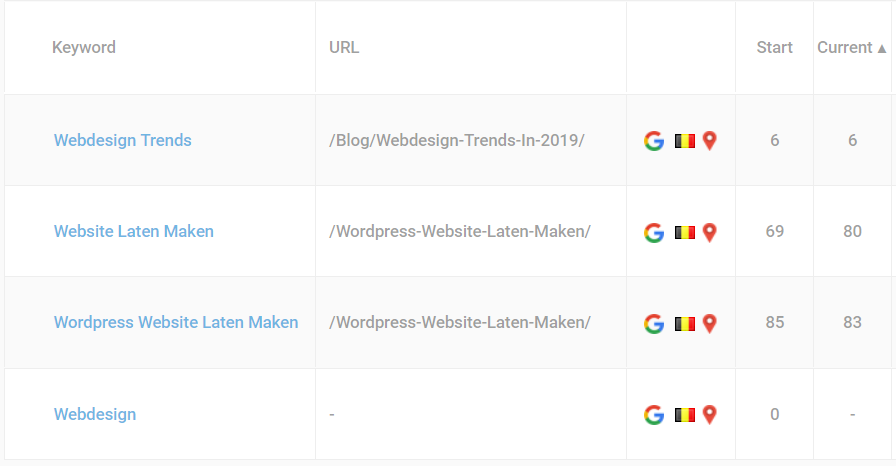
\includegraphics[width=\linewidth]{Bachelorproef/bachelor/img/ranktracker.PNG}
(Een screenshot van de werking van Rank Tracker, eigen zoekwoorden)

Het is ook makkelijk om via 'competitie' te kijken op welke plek de concurrentie (deze websites kan je zelf ingeven) rankt voor een bepaald zoekwoord.

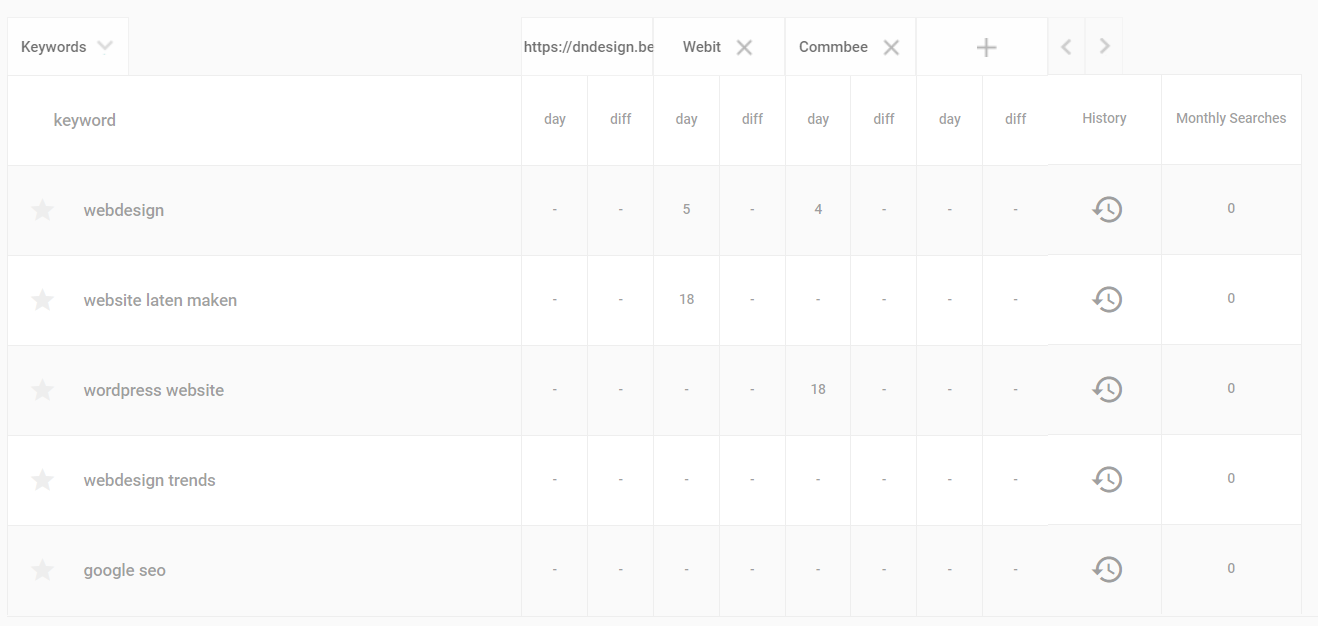
\includegraphics[width=\linewidth]{Bachelorproef/bachelor/img/ranktrackercom.PNG}
(Een screenshot van de werking van Rank Tracker, zoekwoorden van de concurrentie)

Bij de tool kan je zelf de taal en het land instellen. 

\subsubsection{Accuranker}
\label{ch: Accuranker}
Er is een gratis testaccount (zonder kredietkaart) waarbij je voor 14 dagen een trial kan uitproberen. 

De betalende versies: 
\begin{itemize}
\item 78 dollar per maand - tot 1000 keywords
\item 249 dollar per maand - tot 5000 keywords
\item 399 dollar per maand - tot 1750 keywords
\end{itemize}

Je kan zelf de zoekwoorden ingeven voor een bepaalde domeinnaam en de ranking van een zoekwoord vergelijken met een dag, week of maand geleden (het minimum is 2 uur). 

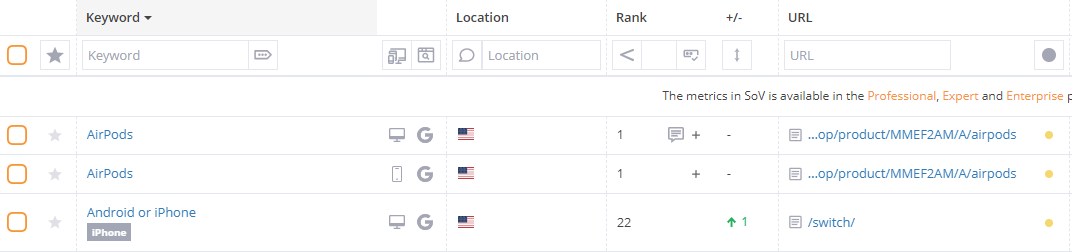
\includegraphics[width=\linewidth]{Bachelorproef/bachelor/img/accuranker.PNG}
(Een screenshot van de werking van Accuranker, eigen zoekwoorden)

Het is makkelijk om te vergelijken met de concurrentie. Op het overzicht zie je duidelijk welke keywords omhoog gegaan zijn in vergelijking met de concurrentie, en welke gezakt zijn. 

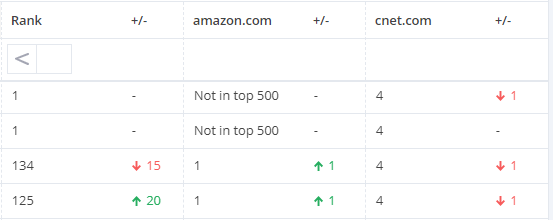
\includegraphics[width=\linewidth]{Bachelorproef/bachelor/img/accurankercompetitie.PNG}
(Een screenshot van de werking van Accuranker, zoekwoorden van de concurrentie)

Bij elk pakket kan je een ongelimiteerd aantal domeinen gebruiken. 

Bij de tool kan je zelf de taal en het land instellen. 

\subsection{Overzicht}
\label{ch: Overzicht}

In de volgende tabel wordt een overzicht gegeven van alle besproken tools. 

Korte legende: 
\begin{itemize}
\item Rood: niet aanwezig in de tool
\item Groen: wel aanwezig in de tool
\end{itemize}

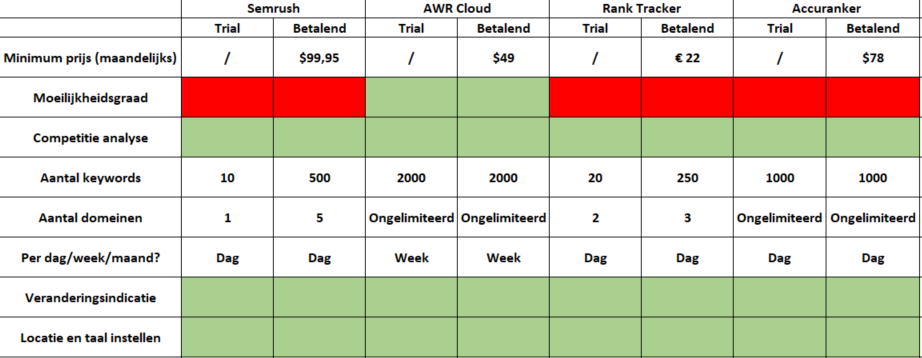
\includegraphics[width=\linewidth]{Bachelorproef/bachelor/img/rankingtabel.PNG}
(Een overzichtelijke tabel met alle functionaliteiten van de ranking tools)

Alle tools bieden een korte trial of probeerversie aan. Semrush is de enige tool die niet automatisch betalend wordt na verloop van tijd. De functionaliteiten zijn dezelfde als bij de andere tools met uitzondering dat de moeilijkheidsgraad voor een keyword wordt aangegeven bij AWR Cloud. De trial versie van AWR Cloud duurt 30 dagen. De beste gratis tool is dus Semrush omdat deze gratis blijft. 

Voor de betalende versies is te zien dat AWR Cloud de meeste functionaliteiten heeft (groen). Rank Tracker is de goedkoopste tool (vanaf 22 euro) maar er kunnen slechts 250 keywords getrackt worden. In vergelijking met AWR Cloud (vanaf 49 dollar) zijn dit er 2000. Voor eigen gebruik of hele kleine agencies kunnen 250 keywords al genoeg zijn, maar voor een SEO-bureau zoals WiSEO zijn er al snel 2000 of meer keywords nodig. 

We kunnen dus concluderen dat AWR Cloud de beste betalende tool is. 

\section{Linkbuilding tools}
\label{ch: Linkbuilding tools}

\subsection{Doel van een linkbuilding tool}
\label{ch: Doel van een linkbuilding tool}

Het doel van linkbuilding is autoriteit opbouwen binnen de zoekmachine. Als er veel naar een website verwezen wordt met een hyperlink (vanaf een andere site) is het vermoedelijk een interessantere website in vergelijking met een site die geen inkomende links heeft. 

Om het woord autoriteit volledig te kunnen schetsen moeten we terugkeren naar wanneer de term ‘PageRank’ nog van toepassing was. Deze methode ordent pagina’s op het internet volgens belang (definitie op Wikipedia). Het is een cijfer van nul tot tien op basis van het aantal externe links. Google ziet een link van pagina A naar pagina B als een stem. Hoe hoger de PageRank is van pagina A, hoe belangrijker de stem is. 

De PageRank is niet meer zichtbaar sinds 15 april 2016. 

Er kwamen al gauw vervangers voor PageRank, die aan de hand van algoritmes een indicatie geven van de sterkte of autoriteit van een pagina. Er zijn twee tools die waarden aangeven ter vervanging van PageRank, namelijk: Moz (PA en DA) en Majestic (TF en CF). Dit is ook één van de aspecten die zal besproken worden in het onderzoek. 

Linkbuilding is het zorgen voor meer autoriteit binnen een website door strategisch (door het plaatsen van links op websites die meer verkeer naar je eigen website brengen) meer hyperlinks op gerelateerde websites te krijgen (die eventueel al een hoge autoriteit hebben).

\subsection{Geteste aspecten}
\label{ch: Geteste aspecten}

\begin{itemize}
\item Prijs: er zal gekeken worden of er een gratis versie of een tijdelijke trial is en wat de kostprijs van de tool is (maandelijks). Sommige tools hebben beperkingen bij de gratis versie of trial en dit zal duidelijk gemaakt worden in het onderzoek.  
\item Waarde van de domeinnaam en de pagina: wordt er een indicatie gegeven van de waarde (autoriteit) van een bepaalde pagina en/of volledig domein? 
\item Linking domains: wordt er weergegeven welke domeinen (van andere websites) linken naar jouw pagina (of de website waarnaar je onderzoek doet)?
\item Hoeveel domeinen kan je opzoeken per dag?
\item Hoeveel domeinen (backlinks) laat de tool zien?
\item Anchor tekst: dit is de tekst waarop je kan klikken bij een hyperlink. In HTML-code ziet dit er als volgt uit: <a href=”https://dndesign.be/”>webdesign</a> . De anchor tekst is de tekst tussen de > en </a>. Het is belangrijk dat deze tekst relevant is met de pagina waarnaar verwezen wordt. 
\item Spam score: geeft een bepaald percentage terug van websites met gelijkaardige kenmerken die geband worden door Google. Geband betekent een afstraffing van Google waardoor je een slechtere ranking krijgt of volledig uit de zoekresultaten wordt verwijderd. 
\end{itemize}

\subsection{Vergelijkende studie tussen linkbuilding tools}
\label{ch: Vergelijkende studie tussen linkbuilding tools}

De tools die werden vergeleken zijn Ahrefs, Moz Link Explorer, Majestic en backlink-checker. De reden dat deze 4 tools werden uitgekozen is omdat AWR Cloud wordt gebruikt bij WiSEO en ze worden vermeld in deze artikels: \textcite{SEO13} en \textcite{SEOCOMPLETE}.  

\subsubsection{Ahrefs}
\label{ch: Ahrefs}
De tool Ahrefs heeft geen gratis versie. 

Ahref maakt gebruik van een metric namelijk Domain Rating. De Domain Rating is een metric die de sterkte aangeeft van het backlinkfprofiel van een website. Hierbij worden het totaal aantal links en de kwaliteit ervan meegenomen om een score toe te kennen. 

De betalende versies: 
\begin{itemize}
\item 99 dollar per maand - 100 URL's per dag - tot 10000 backlinks per domein
\item 179 dollar per maand - 500 URL's per dag - Tot 30000 backlinks per domein
\item 399 dollar per maand - 2000 URL's per dag - Tot 50000 backlinks per domein
\end{itemize}

Bij het ingeven van je website wordt er een duidelijk overzicht gegeven met de volgende gegevens (de belangrijkste): DR (Domain Rating), aantal links naar je website (Backlinks), aantal domeinen die een link hebben naar je website en een overzichtelijke grafiek die de Ahrefs Rank evolutie toont. 

Ahrefs Rank is een positie in de ranking van Ahrefs die je website krijgt op basis van een aantal factoren. Er wordt en vergelijking gemaakt met alle websites in hun database.

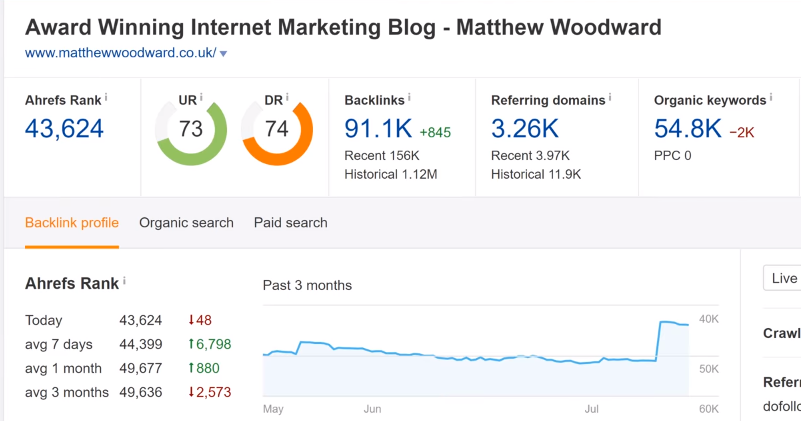
\includegraphics[width=\linewidth]{Bachelorproef/bachelor/img/ahrefs.PNG}
(Een screenshot van het ahrefs programma, de homepagina)

Je kan precies elke pagina zien die een backlink bevat naar je website. De Anchor text wordt telkens getoond.

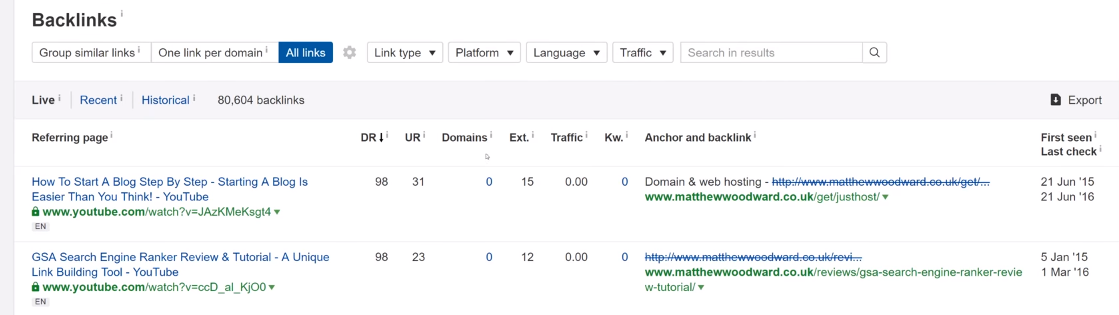
\includegraphics[width=\linewidth]{Bachelorproef/bachelor/img/ahrefsbacklink.PNG}
(Een screenshot van de backlinkpagina waar alle binnenkomende links staan)

Er wordt geen spam score getoond. 

\subsubsection{Backlink-checker}
\label{ch: Backlink-checker}

Deze tool heeft enkel een gratis versie. Er wordt een indicatie gegeven van de waarde van een domein door de Ahrefs Domain Rating, terug te vinden bij de tool Ahref.

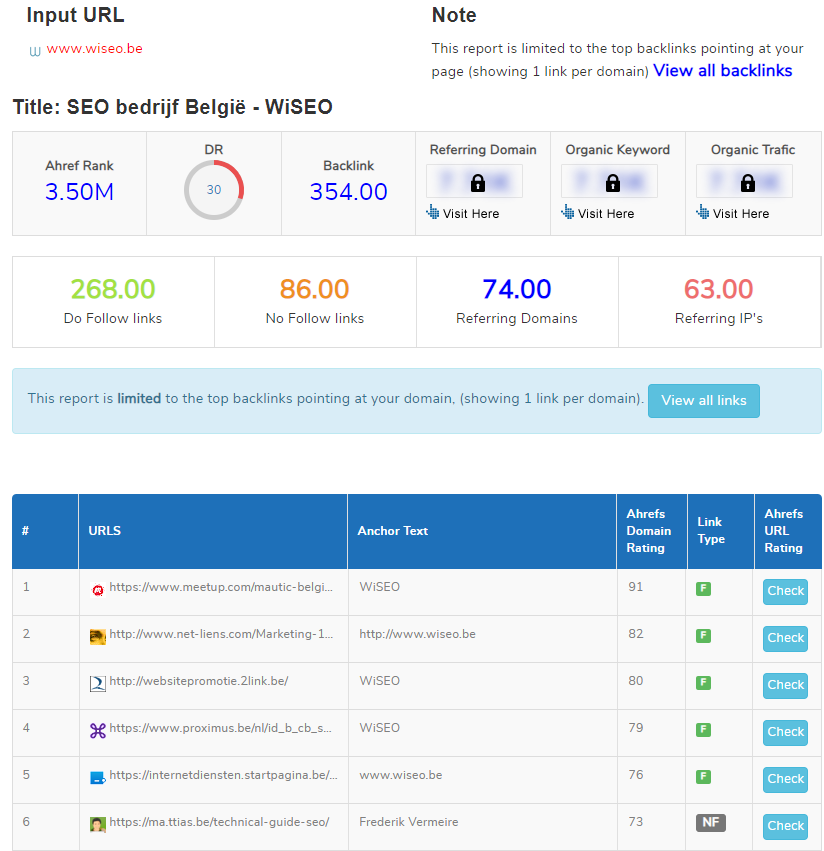
\includegraphics[width=\linewidth]{Bachelorproef/bachelor/img/backlinkchecker.PNG}
(Screenshot van het programma Backlink-Checker)

Per dag kan je een ongelimiteerd aantal domeinen opzoeken waarbij je per domein de eerste 100 domeinen ziet die een backlink voorzien, dit zijn degene met de hoogste Domain Ratings.

De tool geeft een specifieke URL terug van de pagina die een hyperlink heeft naar jouw pagina. De anchortekst wordt ook weergegeven. Er wordt geen spamscore getoond. 

\subsubsection{Majestic}
\label{ch: Majestic}
Er zijn twee metrics afkomstig van de tool Majestic, namelijk Trust Flow(TF) en Citation Flow(CF). Trust Flow is een metric die aangeeft hoe betrouwbaar een website is. Als je bijvoorbeeld een link krijgt van HLN, gaat je Trust Flow omhoog. (Dit omdat HLN een zeer betrouwbare website is.) Citation Flow is een metric die aangeeft hoeveel andere websites naar een bepaalde website verwijzen. (Hoe meer verschillende websites, hoe hoger de CF zal zijn.)

Er is een gratis trial waarbij je tot drie keer een domein kan ingeven, daarna kan je geen websites meer opzoeken en moet je een maandabonnement kopen. Je krijgt enkel de TF en CF te zien.

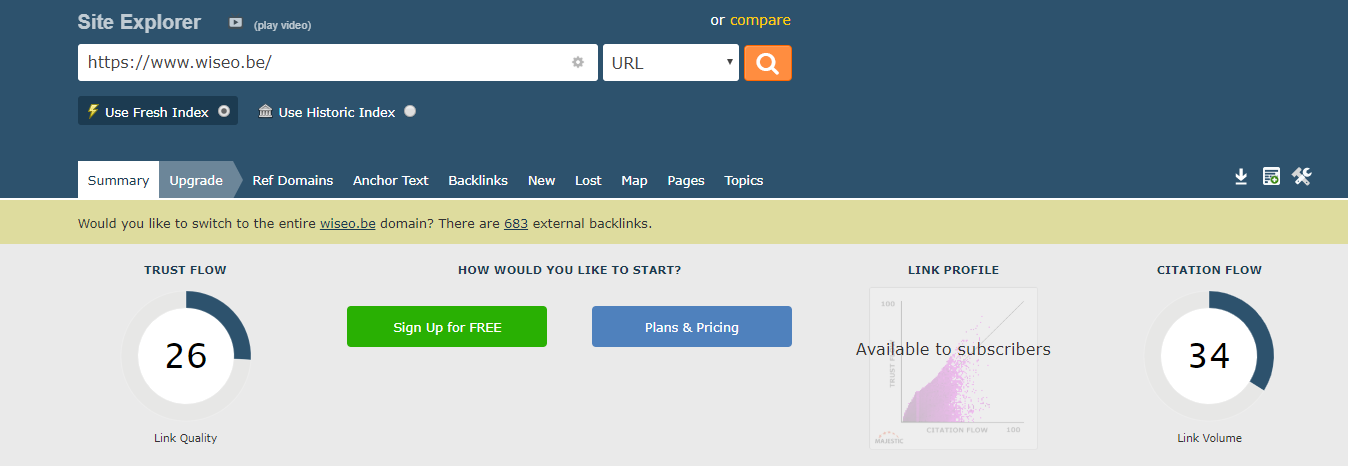
\includegraphics[width=\linewidth]{Bachelorproef/bachelor/img/majesticgratis.PNG}
(Een screenshot van de gratis tool van Majestic)

De betalende versies: 
\begin{itemize}
\item 46,99 euro per maand - Tot 5000 backlinks per domein
\item 94,99 euro per maand - Tot 15000 backlinks per domein
\end{itemize}

Bij de betalende versie kan je de tabbladen gebruiken zoals backlinks, ref domains en anchor text. Bij het tabblad 'backlinks' (deze kan je niet gebruiken bij de gratis versie) zie je alle domeinen die met een link verwijzen naar een bepaalde website. Bij het tabblad 'Anchor Text' kan je de precieze anchor text zien die per link gebruikt wordt. 

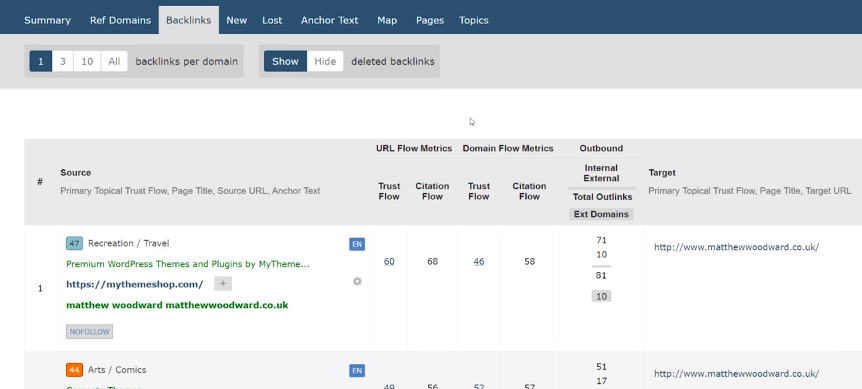
\includegraphics[width=\linewidth]{Bachelorproef/bachelor/img/majesticbacklink.PNG}
(Een screenshot van de betalende tool van Majestic met de backlinks)

Er wordt geen rechtstreekse 'spam score' getoond. 

\subsubsection{Moz Link Explorer}
\label{ch: Moz Link Explorer}

Er zijn twee metrics afkomstig van de tool Moz, namelijk Domain Authority (DA) en Page Authority (PA). Ze hebben een waarde tussen de 1 en 100. Hoe hoger het getal hoe hoger de autoriteit. Enkele factoren van de domeinwaarde (autoriteit) zijn: het aantal links naar je website, het aantal verschillende 'root domains' die naar je website verwijzen en de kwaliteit van de links. Naast DA geeft de tool ook een score aan individuele pagina's, namelijk PA. 

Moz heeft een gratis versie waarbij je tot 10 links kan ingeven per maand. Je kan tot 50 backlinks zien per domein. 

De betalende versies: 
\begin{itemize}
\item 99 dollar per maand - 5000 URL's per maand - Tot 10000 backlinks per domein
\item 179 dollar per maand - 20000 URL's per maand - Tot 40000 backlinks per domein
\item 249 dollar per maand - 70000 URL's per maand - Tot 50000 backlinks per domein
\end{itemize}

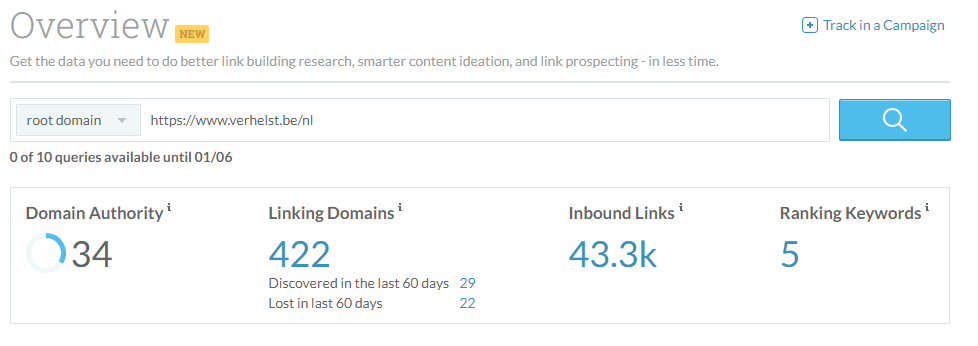
\includegraphics[width=\linewidth]{Bachelorproef/bachelor/img/mozbacklink.PNG}
(Een screenshot van de overview pagina van Moz)

De tool laat zien welke domeinen linken naar je eigen pagina (of de website waarnaar je onderzoek doet). De anchortekst wordt duidelijk weergegeven. 

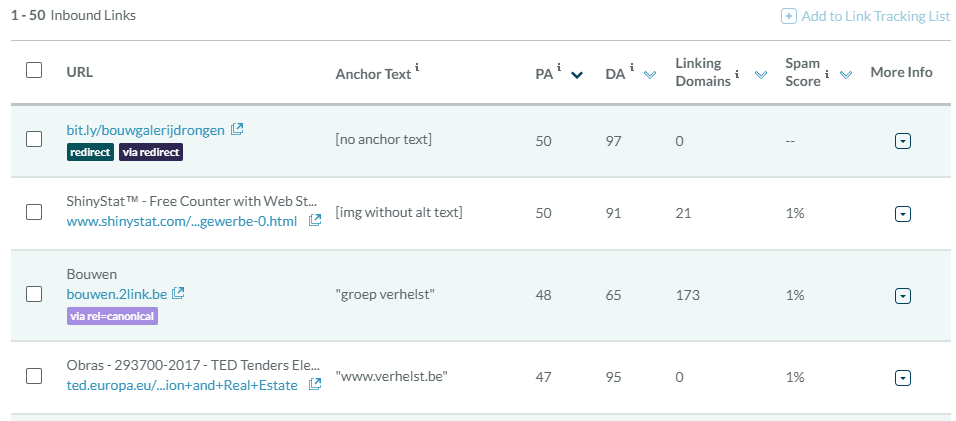
\includegraphics[width=\linewidth]{Bachelorproef/bachelor/img/mozbacklinks.PNG}
(Screenshot van de gedetailleerde pagina van Moz die alle backlinks laat zien)

Als laatste wordt er een spam score aangegeven. Moz zegt hierover het volgende: "vertegenwoordigt het percentage sites met vergelijkbare functies waarvan we hebben vastgesteld dat ze bestraft of verbannen zijn door Google".

\subsection{Overzicht}
\label{ch: Overzicht}

In de volgende tabel wordt een overzicht gegeven van alle besproken tools. 

Korte legende: 
\begin{itemize}
\item Rood: niet aanwezig in de tool
\item Groen: wel aanwezig in de tool
\end{itemize}

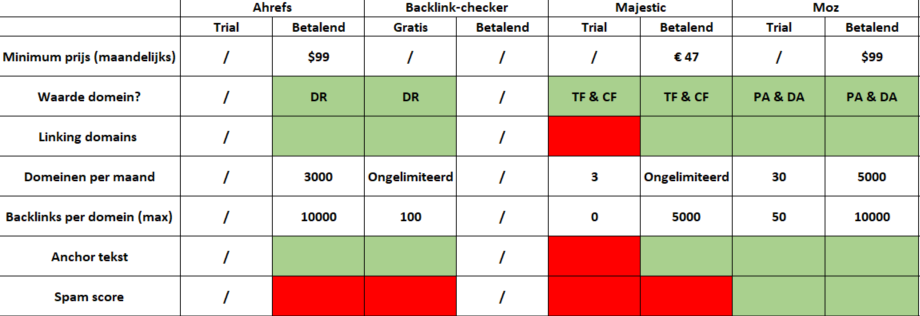
\includegraphics[width=\linewidth]{Bachelorproef/bachelor/img/linkbuildingtabel.PNG}
(Een overzichelijke tabel waar alle functionaliteiten instaan van backlink tools)

De beste gratis tool is Backlink-Checker. Deze tool heeft, in vergelijking met Majestic (3 per maand) en Moz (10 per maand), een ongelimiteerd aantal domeinen die je kan opzoeken. Er worden bij de Backlink-checker ook tot 100 links per domein getoond. Het enige nadeel is dat er geen spam score wordt weergegeven zoals bij Moz. 

Als betalende tool kan je afleiden dat Majestic de beste tool is.

Enkele argumenten: 
\begin{itemize}
\item Het is de goedkoopste tool.
\item Er kan een ongelimiteerd aantal domeinen per maand opgezocht worden. 
\item 5000 backlinks per domein in tegenstelling tot 10000 bij de andere tools. Er zijn weinig websites die meer dan 5000 backlinks hebben.
\item Er wordt enkel een spamscore getoond bij Moz, maar dit artikel, \textcite{MAJESTIC} , toont aan dat je aan de hand van TF en CF ook een indicatie van de spamscore (Trust ratio) krijgt. 
\item Op de andere vlakken komt het overeen met de andere tools.
\end{itemize}

\section{Technische tools}
\label{ch: Technische tools}

\subsection{Doel van een technische tool}
\label{ch: Doel van een technische tool}

Eén van de voorwaarden om goed te kunnen scoren in zoekmachines is zorgen dat de technische kant van je site in orde is. Het is één van de basiselementen voor SEO. Vaak worden fouten gemaakt waardoor bijvoorbeeld links niet meer werken of de URL-structuur van de website niet in orde is (wordt uitgelegd bij de geteste aspecten). Omdat je website fouten bevat kan Google je daarvoor afstraffen en laten dalen in de zoekresultaten. 

De zoekmachine Google maakt gebruik van crawlers, dit heet de GoogleBot. Webcrawlers zijn stukken software waarmee alle pagina’s op je website doorzocht worden en op die manier alle pagina’s gaat indexeren (het registreren van pagina’s in hun database). 

Het is van cruciaal belang dat de website een goede hiërarchie bevat met links naar onderliggende pagina’s. Dit ziet er bijvoorbeeld als volgt uit: 

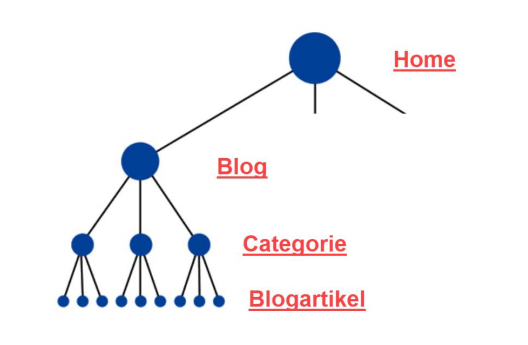
\includegraphics[width=\linewidth]{Bachelorproef/bachelor/img/Websitestructuur.png}
(Een afbeelding die een voorbeeld geeft van een websitehiërarchie)

Een hiërarchische structuur is maar één van de vele aspecten op technisch vlak. Bij de geteste aspecten worden deze allemaal duidelijk uitgelegd.

Bij WiSEO neemt het maken van technische audits een veel tijd in beslag. Op hun SEO-auditpagina staat meer uitleg over de werkwijze. \textcite{AUDIT} 

Bij dit onderzoek van technische tools zal de nadruk liggen op tools die een volledige website crawlen, zoals de GoogleBot, en hier allerlei informatie uit afleiden.

Een SEO-crawler is een tool die makkelijk door elke pagina gaat op een website en alle nodige informatie afleidt. Door deze tools hoef je niet langer handmatig op elke pagina te klikken op je website om titels, headers, interne links, … te controleren. Het scheelt dus veel tijd en is overzichtelijk. 


\subsection{Geteste aspecten}
\label{ch: Geteste aspecten}

Deze aspecten zijn vooral gebaseerd op basis van de technische audits die opgemaakt worden door WiSEO.

\begin{itemize}
\item Prijs: er zal gekeken worden of er een gratis versie of een tijdelijke trial is en wat de kostprijs van de tool is (maandelijks). Sommige tools hebben beperkingen bij de gratis versie of trial en dit zal duidelijk gemaakt worden in het onderzoek. 
\item Desktop of cloud: 
desktop crawlers zijn crawlers die geïnstalleerd worden op je eigen PC. In het algemeen zijn deze veel goedkoper maar ze hebben wat beperkingen. De grootste beperking is dat ze veel geheugen en CPU verbruiken van een PC of laptop. In de bedrijfsomgeving (zoals WiSEO) kan je niet simpelweg een rapport delen met een klant of collega maar moet je eerst het bestand downloaden en zo het project doorsturen. 

Cloud crawlers zijn vaak duurder dan desktop crawlers. Bij de meeste kun je simpelweg toegang verlenen aan klanten of collega’s zodat ze de resultaten kunnen zien. Over het algemeen zijn ze krachtiger dan desktop crawlers. 

\item Metagegevens: dit bestaat uit de meta-title en de meta-description. Dit is belangrijk om een potentiële bezoekers aan te trekken zodat ze sneller op de link klikken. Via deze technische tools krijg je een duidelijk overzicht per pagina wat de metagegevens zijn. Een voorbeeld (rood is de meta-title en blauw is de meta-description):

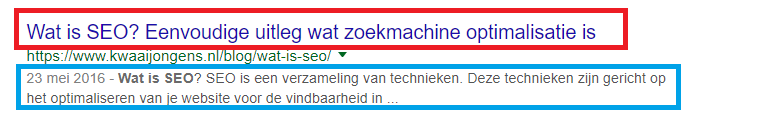
\includegraphics[width=\linewidth]{Bachelorproef/bachelor/img/metadescription.png}
(Een voorbeeld van een meta-title en meta-description in Google)

\item Header tags: geeft de tool de header tags terug van alle pagina’s voor een bepaalde website. Dit kunnen we zien als tekst die tussen de <h1>..</h1>, <h2>..</h2> en <hx>..</hx> tags staan. Voor elke pagina is dit noodzakelijk omdat Google kijkt naar de headers om de structuur van een pagina beter te begrijpen.  
\item Duplicated content: duplicated content is content op twee of meer pagina’s die gelijk aan elkaar zijn (op dezelfde website). Dit wordt afgeraden omdat Google dit kan afstraffen. Het is daarom ook belangrijk om te weten of dit het geval is zodat je dit kan oplossen. 
\item Crawl depth: geeft de tool informatie weer over de crawl depth of het aantal klikt dat je nodig hebt voor een bepaalde pagina, vanaf de homepage. Als bijvoorbeeld een belangrijke pagina niet bereikbaar is in één of twee kliks van je homepage kan dit aangeven dat je website een slechte structuur heeft.  
\item Interne links: geeft een lijst terug van alle interne links. Dit zijn links van van één pagina naar een andere binnen dezelfde website. Tools kunnen dan aangeven of er genoeg interne links zijn naar een bepaalde pagina en als ze correct werken. 
\item Outbound links (externe links): geeft een lijst terug van alle externe links (link van de ene website naar een andere). 
\item Pagespeed: de laadtijd van een website is heel belangrijk voor zowel gebruikers als de SEO. Wordt er een indicatie gegeven van de snelheid en wat er kan veranderen om dit te verbeteren? 
\item Responsive test: geeft de tool aan of de website responsive in orde is of niet? Voor Google is het belangrijk dat een site responsive is en zich dus kan aanpassen op alle toestellen (desktop, tablet en mobiel). 
\end{itemize}

\subsection{Vergelijkende studie tussen technische tools}
\label{ch: Vergelijkende studie tussen technische tools}

De tools die worden vergeleken zijn Screaming Frog, Sitebulb, DeepCrawl, OnCrawl en Website Auditor. De reden dat deze 5 tools werden uitgekozen is omdat Screaming Frog en OnCrawl worden gebruikt bij WiSEO en ze worden vermeld in deze artikels: \textcite{SEO13} en \textcite{SEOCOMPLETE}.  

\subsubsection{Screaming Frog}
\label{ch: Screaming Frog}

Screaming Frog heeft een gratis versie waarbij je tot 500 URL's kan crawlen per website, dit heet het 'crawl limiet'. 

Er is maar 1 betalende versie, je kan een ongelimiteerd aantal URL's crawlen voor de prijs van £149 per jaar. 

Screaming Frog is een desktop crawler. De gegevens zoals metagegevens, header tags, crawl depth, interne links en outbound links zijn makkelijk terug te zien. 

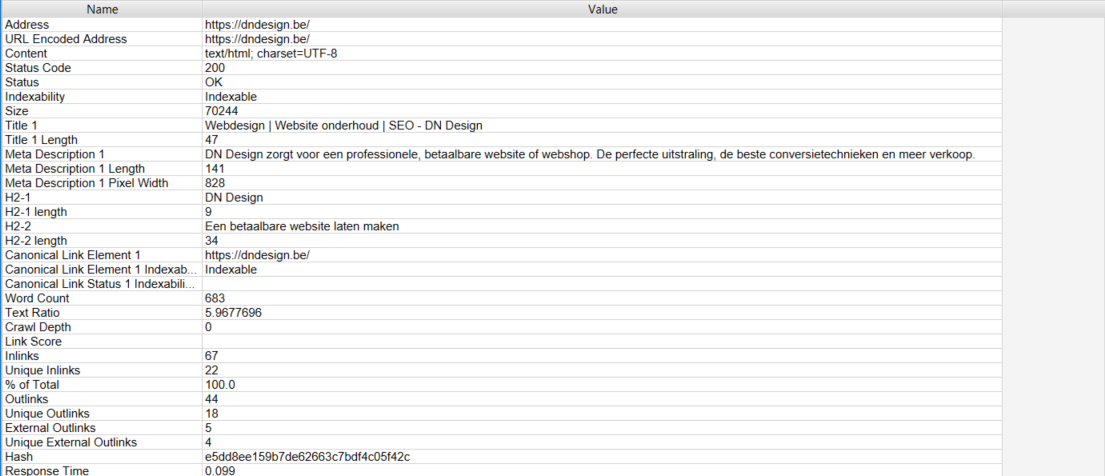
\includegraphics[width=\linewidth]{Bachelorproef/bachelor/img/screamingfrog.PNG}
(Een screenshot van het programma Screamingfrog)

Er wordt ook aangegeven of er duplicate content aanwezig is op de website. 

\subsubsection{Sitebulb}
\label{ch: Sitebulb}

Sitebulb is een relatief nieuwe tool op de markt. Omdat Sitebulb een desktop-software is, kun je niet zomaar een rapport delen met je collega's tijdens een SEO-audit. Je kan dit gedeeltelijk omzeilen door een rapport naar PDF te exporteren. Zodra je op de knop "Exporteren" klikt, zie je een document van 40 pagina's, vol met grafieken, met de belangrijkste inzichten. Het is een dekstop crawler. 

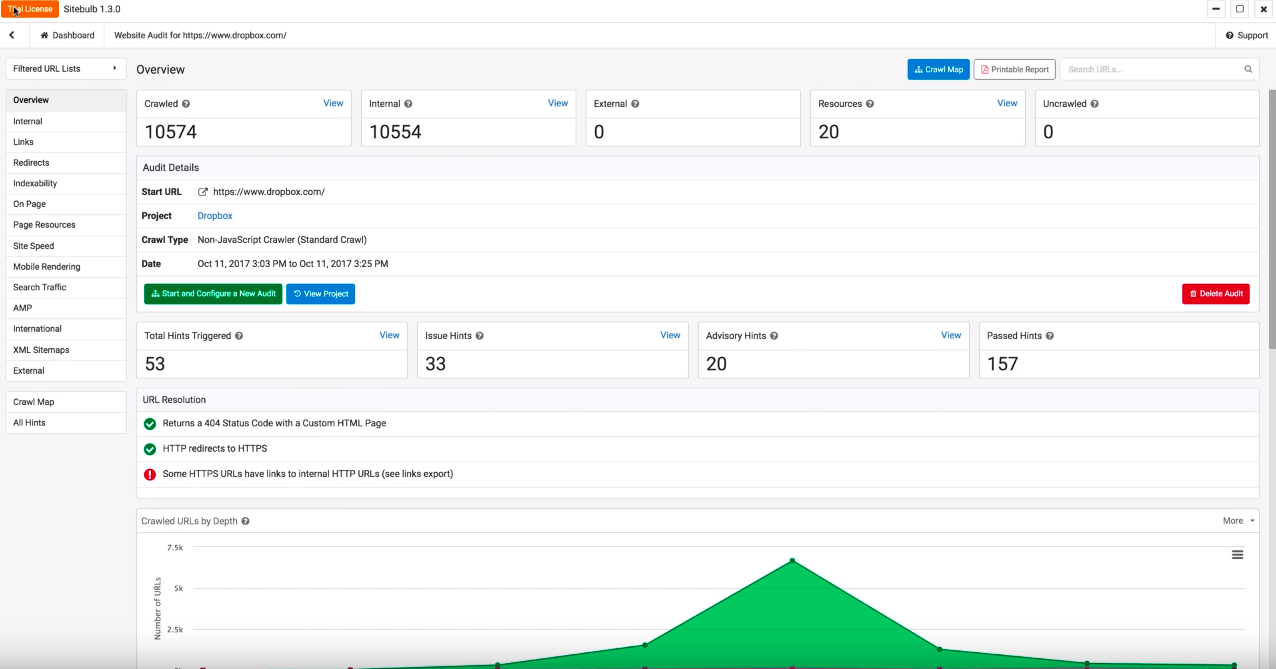
\includegraphics[width=\linewidth]{Bachelorproef/bachelor/img/sitebulb.PNG}
(Een screenshot van het programma sitebulb, overview pagina)

Er is een trial van 14 dagen die dezelfde functionaliteiten heeft als de betalende versie. 

De betalende versie kost 29 euro per maand. Per audit kunnen er tot 2 miljoen URL's gecrawld worden. 

De tools laat de volgende zaken zien: metagegevens, H1 tag, duplicated content, crawl depth, interne links, externe links, pagespeed en mobile test. 

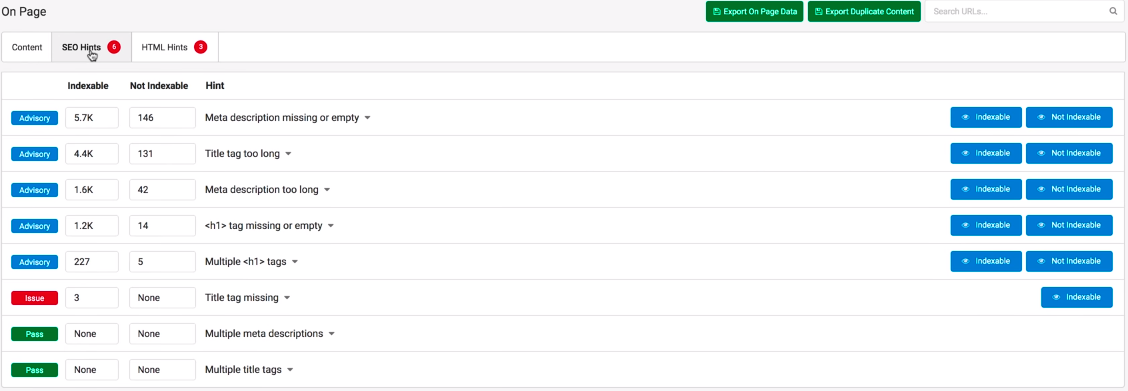
\includegraphics[width=\linewidth]{Bachelorproef/bachelor/img/sitebulb2.PNG}
(Een screenshot van het programma sitebulb, gedetailleerde pagina)

Er is geen informatie aanwezig over H2 tags.

\subsubsection{DeepCrawl}
\label{ch: DeepCrawl}
Er is een gratis trial van 14 dagen waar je tot 1000 URLs kan indexeren.

DeepCrawl is een cloud crawler. 

De betalende versies: 
\begin{itemize}
\item 89 dollar per maand - tot 100 000 URLs - Tot 5 projecten
\item 139 dollar per maand - tot 200 000 URLs - Tot 8 projecten
\end{itemize}

Bij DeepCrawl kan je de metagegevens, header tags, duplicated content, crawl depth, interne en externe links zien. 

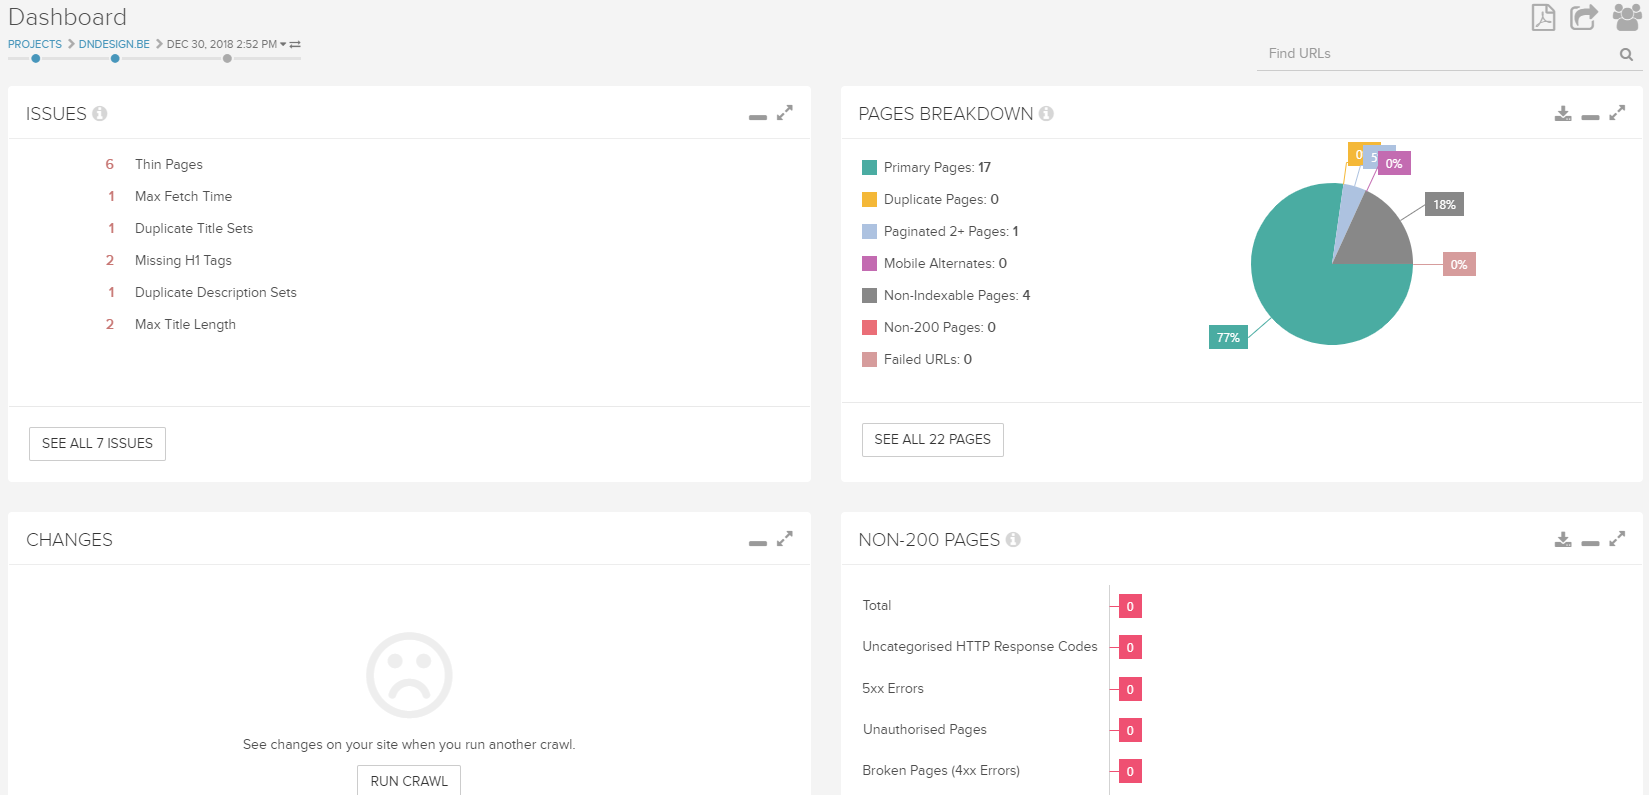
\includegraphics[width=\linewidth]{Bachelorproef/bachelor/img/deepcrawl.PNG}
(Een screenshot van het programma Deepcrawl)

Eén van de grootste nadelen van de tool DeepCrawl is dat je geen extra kolommen aan een rapport kunt toevoegen. Als je bijvoorbeeld een rapport bekijkt dat statuscodes bevat en ook canonieke tags wilt zien, kan je dit niet doen in DeepCrawl. Daarvoor moet je overschakelen naar het canonieke rapport.

Bij de tool worden ook een mobile test en een performance test uitgevoerd.

\subsubsection{OnCrawl}
\label{ch: OnCrawl}
De tool heeft geen gratis versie die je kan uitproberen. 

OnCrawl is een cloud crawler. 

OnCrawl is een cloudgebaseerd hulpmiddel. Hoewel deze tool gericht is naar grotere bedrijven (omwille van de prijs), biedt deze ook een startersplan aan tegen een redelijke prijs. 

Het handige aan deze tool is dat je URL-segmentatie hebt. Indien je bijvoorbeeld een lijst bekijkt met niet-geïndexeerde URL's, kan je gebruik maken van de URL-segmentatie om enkel de blogpagina's te bekijken. 

De betalende versies: 
\begin{itemize}
\item 39 euro per maand - tot 100 000 URLs - Tot 1 project
\item 199 euro per maand - tot 500 000 URLs - Tot 10 projecten
\item 299 euro per maand - tot 2 000 000 URLs - Tot 50 projecten
\end{itemize}

Bij Oncrawl kan je de metagegevens, header tags, duplicated content, crawl depth, interne en externe links zien. 

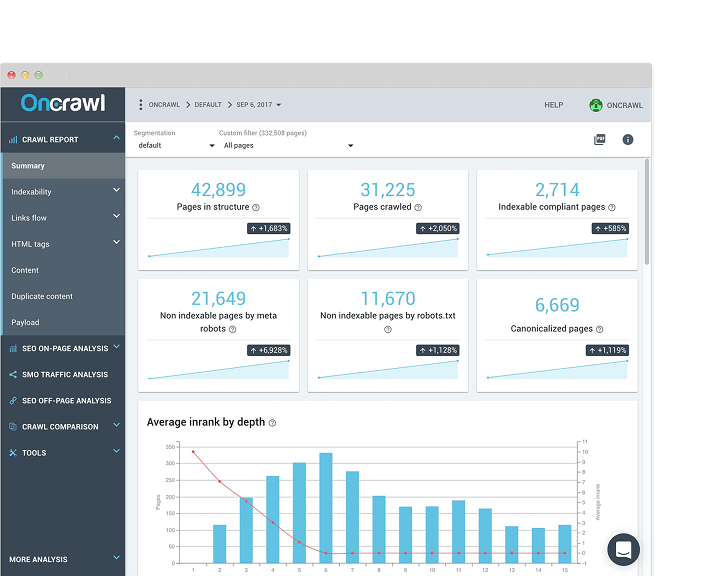
\includegraphics[width=\linewidth]{Bachelorproef/bachelor/img/crawl-report.png}
(Een screenshot van het overzichtsrapport van de tool Oncrawl)

OnCrawl voorziet ook een handig overzicht van de 'link doorstroming' tussen pagina groepen: 

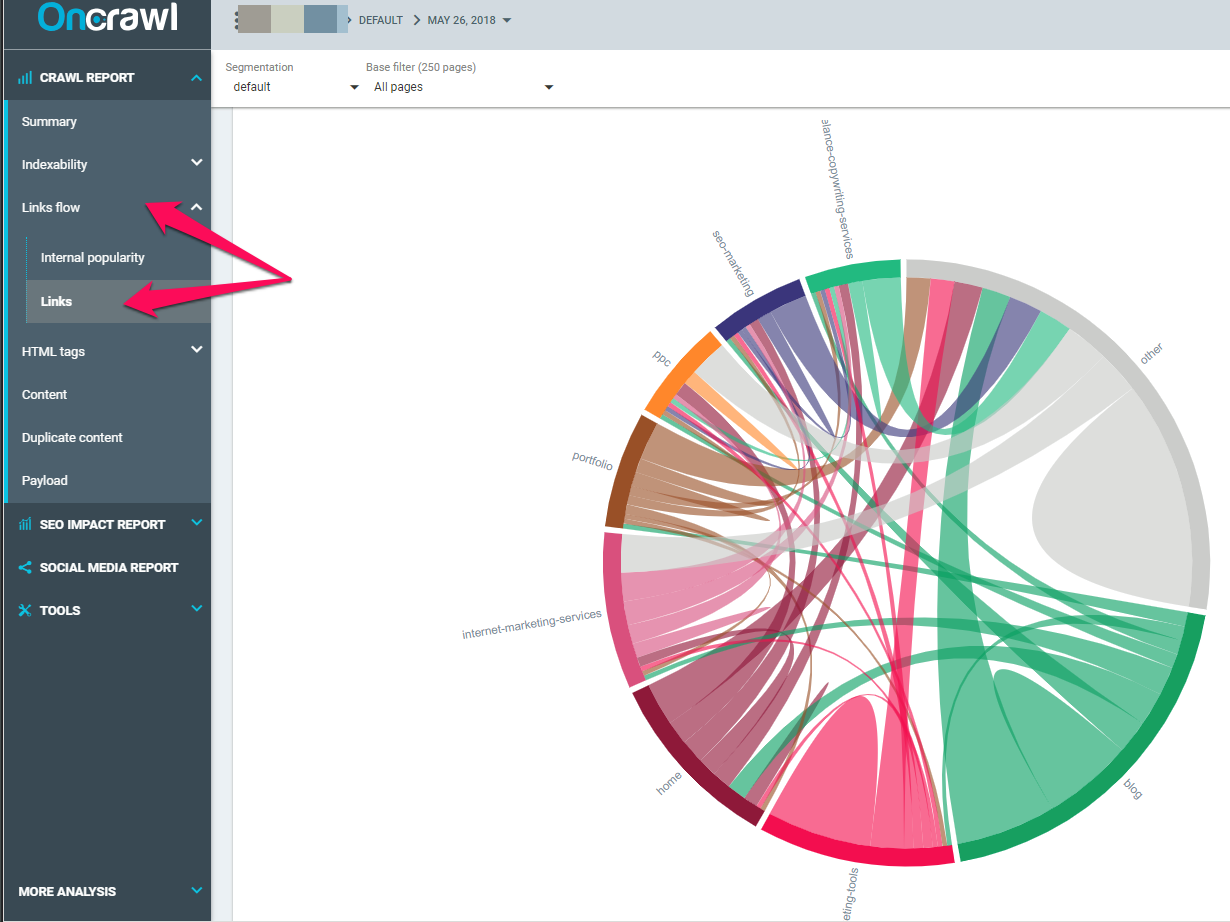
\includegraphics[width=\linewidth]{Bachelorproef/bachelor/img/oncrawl-link-visualization.png}
(Een screenshot van de tool Oncrawl die de link doorstroming laat zien)

\subsubsection{Website Auditor}
\label{ch: Website Auditor}

Website Auditor is een desktop crawler. 

De tool heeft een gratis versie waarbij tot 500 URL's kan crawlen. 
De betalende versies: 
\begin{itemize}
\item 124,75 euro per jaar - Tot 5 projecten
\item 299,75 euro per jaar - Tot 100 projecten
\end{itemize}

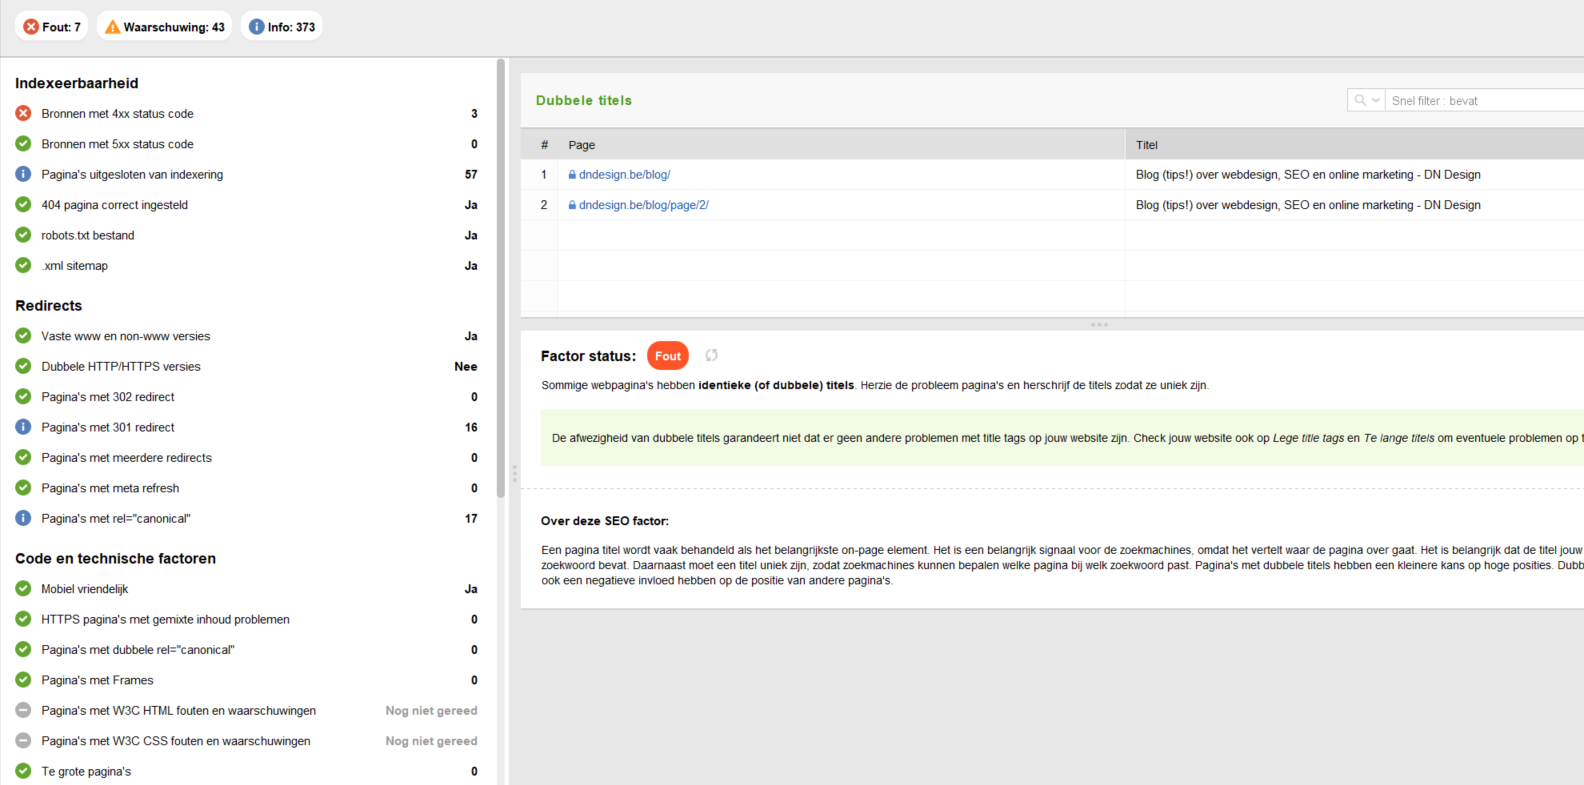
\includegraphics[width=\linewidth]{Bachelorproef/bachelor/img/websiteauditor.PNG}
(Screenshot 1 van de tool Websiteauditor)

Bij Oncrawl kan je de metagegevens, header tags, duplicated content, crawl depth, interne en externe links zien. De tool geeft ook aan of de website mobielvriendelijk is.

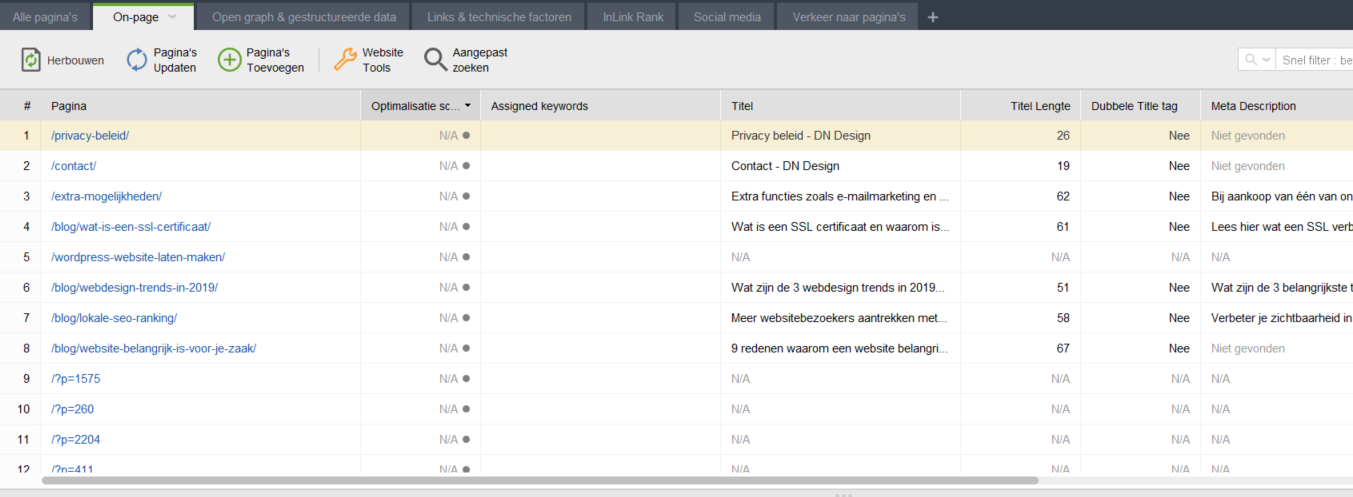
\includegraphics[width=\linewidth]{Bachelorproef/bachelor/img/websiteauditor1.PNG}
(Screenshot 2 van de tool Websiteauditor)

\subsection{Overzicht}
\label{ch: Overzicht}

In de volgende tabel wordt een overzicht gegeven van alle besproken tools. 

Korte legende: 
\begin{itemize}
\item Rood: niet aanwezig op de tool
\item Groen: wel aanwezig op de tool
\end{itemize}

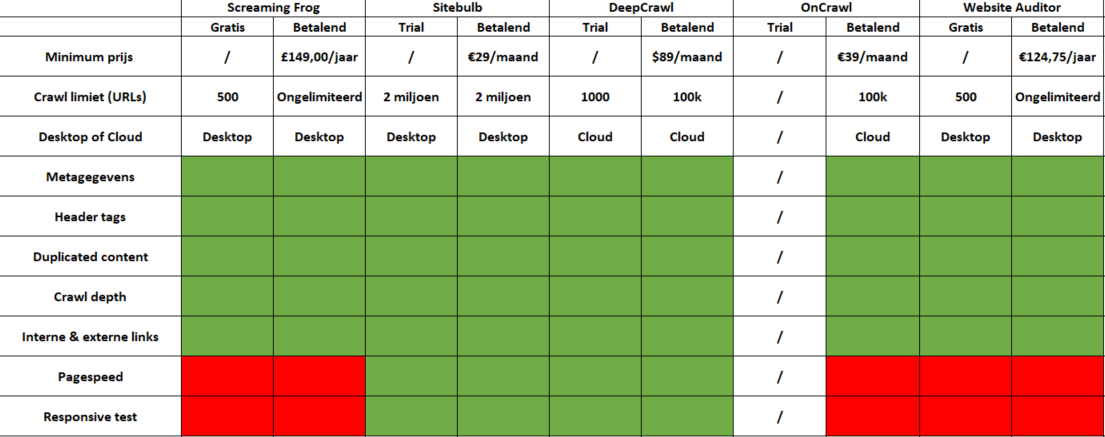
\includegraphics[width=\linewidth]{Bachelorproef/bachelor/img/Knipsel.PNG}
(Overzichtelijke tabel waar alle functionaliteiten instaan van de geteste technische tools)

Afhankelijk van wat je precies met de technische tool wil bereiken, kan je kiezen uit een desktop of cloud crawler. 

Een desktop crawler is beperkt in de zin dat de crawler op je PC zelf staat en je geen online rapport kan delen met klanten of collega's. De prijs is dan wel ook goedkoper dan een cloud crawler. 

Sitebulb heeft de meeste URL's die je kan crawlen (tot 2 miljoen), maar de trial duurt slechts 14 dagen. Om op langere termijn (gratis) een technische tool te gebruiken zijn Screaming Frog of Website Auditor betere opties. 

Sitebulb is de duurste desktop crawler. Indien je bereid bent te betalen voor een technische tool, is het beter om Screaming Frog of Website Auditor te kiezen. Website Auditor is iets goedkoper dan Screaming Frog en is daarom de beste desktop crawler om te gebruiken.

Een cloud crawler bewaart alles online en maakt overzichtelijke rapporten die je kan delen met een klant of collega. 

DeepCrawl heeft een gratis trial van 14 dagen die je kan uitproberen. OnCrawl heeft geen gratis trial. 

De twee tools komen op alle vlakken overeen, behalve de pagespeed en responsive test. Deze zijn niet mogelijk bij OnCrawl. Deze twee tests zijn makkelijk uit te voeren via tools van Google (Pagespeed Insights en Mobile friendly test). De tool OnCrawl is veel goedkoper dan DeepCrawl, dus de voorkeur voor de beste cloud crawler gaat uit naar OnCrawl. 
\chapter{Verbetering van een keyword tool}
\label{ch:tool}

\section{Motivatie}
\label{ch: Motivatie}

Een zoekwoordonderzoek bestaat er onder andere in alle gevonden zoekwoorden onder te verdelen in groepen of clusters. Om het concept  'clusters' te verduidelijken, werken we met een voorbeeld.

Wanneer we bepaalde gerelateerde zoekwoorden en hun zoekvolume te zien krijgen, ziet dit er als volgt uit (wanneer we zoeken op ‘restaurant Brugge’): 

\begin{figure}[h!]
\centering
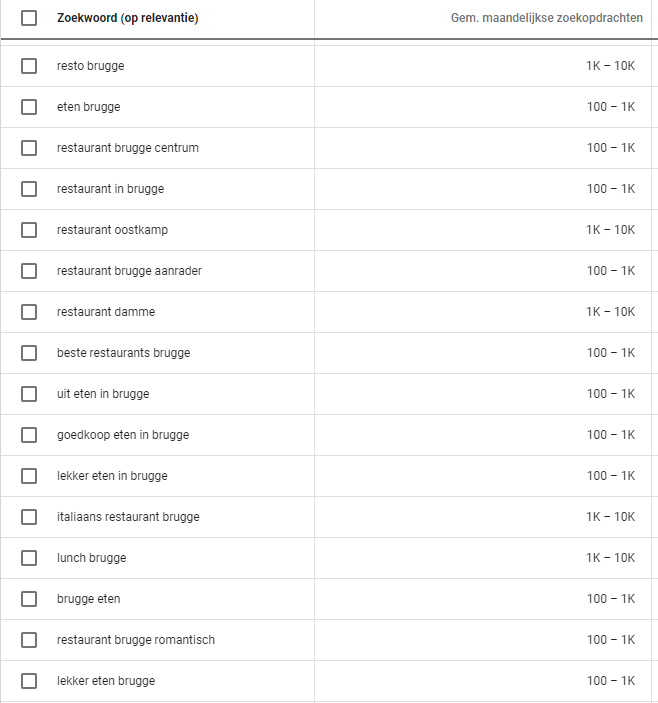
\includegraphics[width=\linewidth]{img/Keywordplannervoorbeeld.png}
\caption{Screenshot van de Zoekwoordplanner die zoekwoordsuggesties geeft voor het zoekwoord 'restaurant Brugge'}
\end{figure}

Er zijn vaak honderden, soms zelfs duizenden zoekwoorden. Om meer overzicht te krijgen hierin, is het een goed idee om dezelfde patronen te groeperen. De zoekwoorden ‘eten Brugge’, ‘uit eten in Brugge’ en ‘Brugge eten’ behoren allemaal tot dezelfde groepering (omdat de intenties van het zoekwoord dezelfde zijn). Van deze zoekwoorden kan je dan een clustergroep maken (van alle mensen die willen eten in Brugge). Die ziet eruit als volgt:

Clustergroep: eten Brugge
eten Brugge - 880
Brugge eten - 390
uit eten in Brugge - 1000

Er bestaan uiteraard nog meer  clustergroepen voor relevante woorden van het keyword ‘restaurant Brugge’. 

Met de zoekwoorden uit deze clustergroepen kan je uiteindelijk landingspagina’s (een pagina op een website) gaan maken, die deze woorden bevatten. Over het algemeen wordt er per clustergroep een landingspagina opgesteld.  

Bij WiSEO gebeurt dit telkens handmatig door middel van Spreadsheets, waarbij alles manueel overgetypt wordt. Vanuit de zoekwoordtool (zie bovenstaande foto) wordt alles één voor één overgenomen. Een voorbeeld van het resultaat: 

\begin{figure}[h!]
\centering
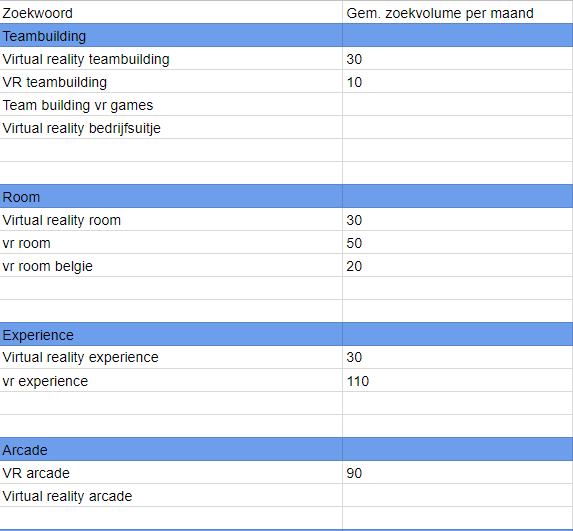
\includegraphics[width=\linewidth]{img/Clustergroepenvoorbeeld.png}
\caption{Voorbeeld van clustergroepen in een Excel bestand}
\end{figure}

\section{Aanpak}
\label{ch: Aanpak}

WiSEO's idee was om een eigen tool te programmeren zodat het proces vergemakkelijkt wordt (en dus minder tijd in beslag neemt), met als doel het handmatige proces van kopiëren en plakken achterwege te laten. 

De werking van deze tool werd gebaseerd op een reeds bestaande tool, namelijk Kwfinder. Het is de bedoeling om een zoekwoord samen in te geven met een bepaald land en een bepaalde taal, om op die manier suggesties te krijgen van gerelateerde zoekwoorden en hun maandelijks zoekvolume. Bij Kwfinder ziet dit er als volgt uit: 

\begin{figure}[h!]
\centering
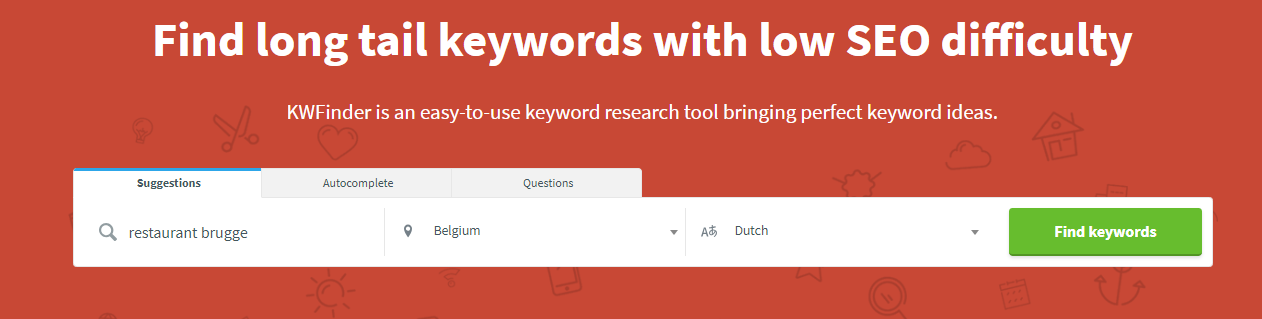
\includegraphics[width=\linewidth]{img/kwfindervoorbeeld.png}
\caption{Screenshot 1 van de tool Kwfinder}
\end{figure}

Na op de knop ‘Find keywords’ te klikken, verkrijg je het volgende resultaat: 

\begin{figure}[h!]
\centering
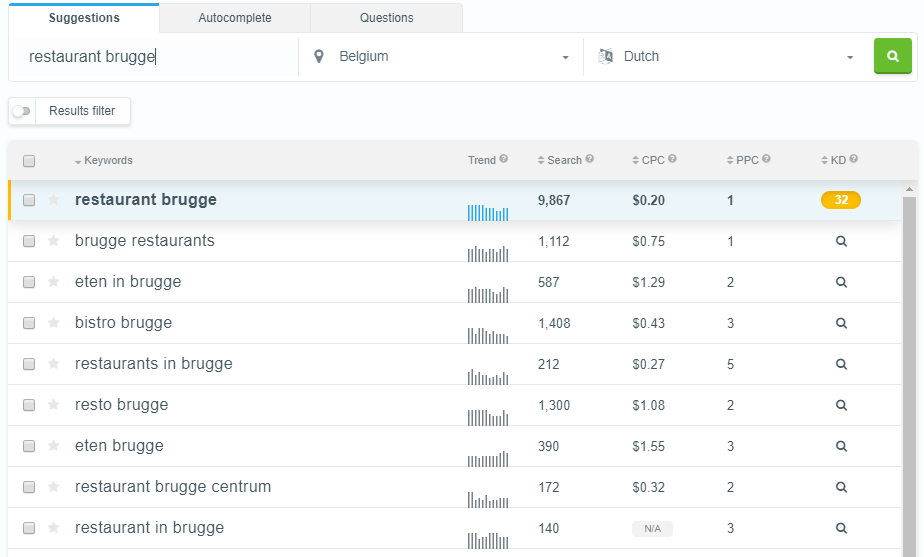
\includegraphics[width=\linewidth]{img/kwfindervoorbeeld2.png}
\caption{Screenshot 2 van de tool Kwfinder}
\end{figure}

De zoekwoordsuggesties en zoekvolumes zijn nu zichtbaar, deze moeten geclusterd worden. De linkerkant van het programma wordt gebaseerd op de bovenstaande foto. 

Clusters en hun zoekwoorden worden ingegeven aan de rechterkant van het programma. Door de zoekwoorden te selecteren (links) kan je ze aan de rechterkant samenvoegen met het zoekvolume in een aangemaakte cluster. 

Om alles te verduidelijken is hieronder een mock-up te vinden van hoe het programma er uit zal zien. Deze mock-ups zijn vooraf gemaakt om het verschil te laten zien tussen het initieel ontwerp en het uiteindelijke product. 

Hier kan je een zoekwoord ingeven met een land en taal naar keuze om zo gerelateerde keywords en het zoekvolume te verkrijgen: 

\begin{figure}[h!]
\centering
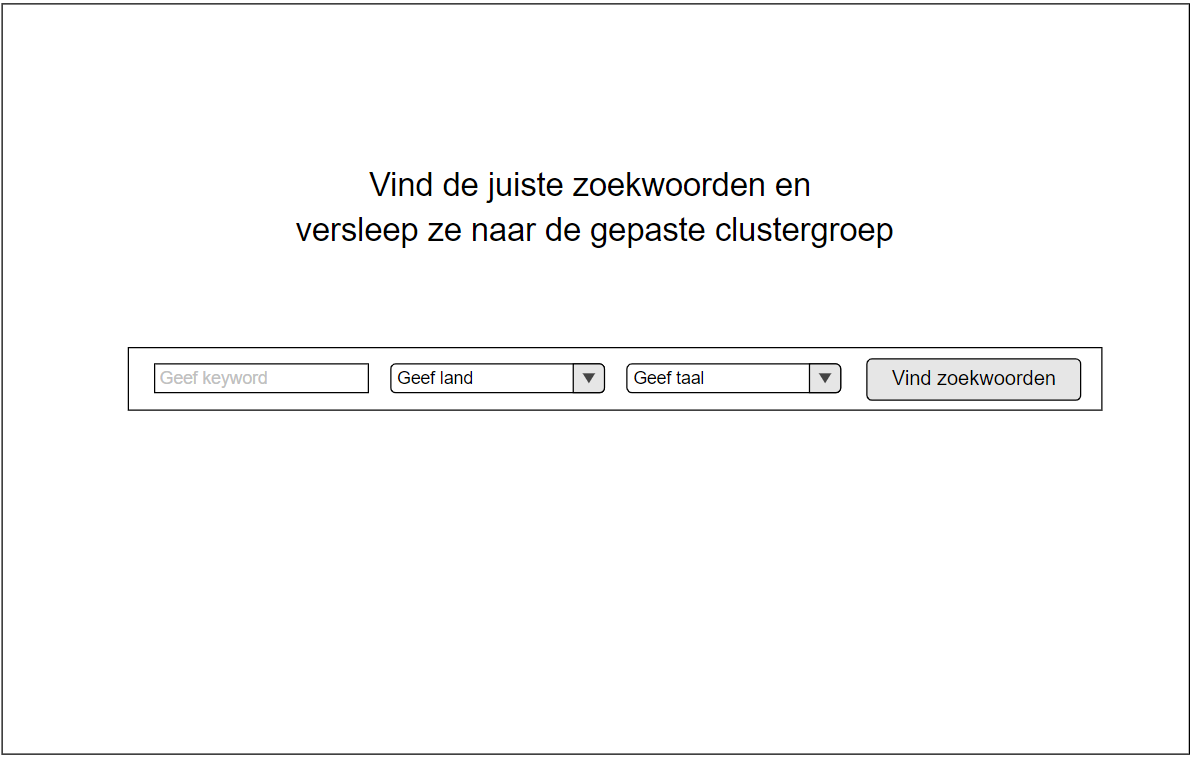
\includegraphics[width=\linewidth]{img/Mockup.png}
\caption{Screenshot van mock-up 1}
\end{figure}

Na op de knop ‘Vind zoekwoorden’ te klikken, verkrijg je het volgende resultaat: 

\begin{figure}[h!]
\centering
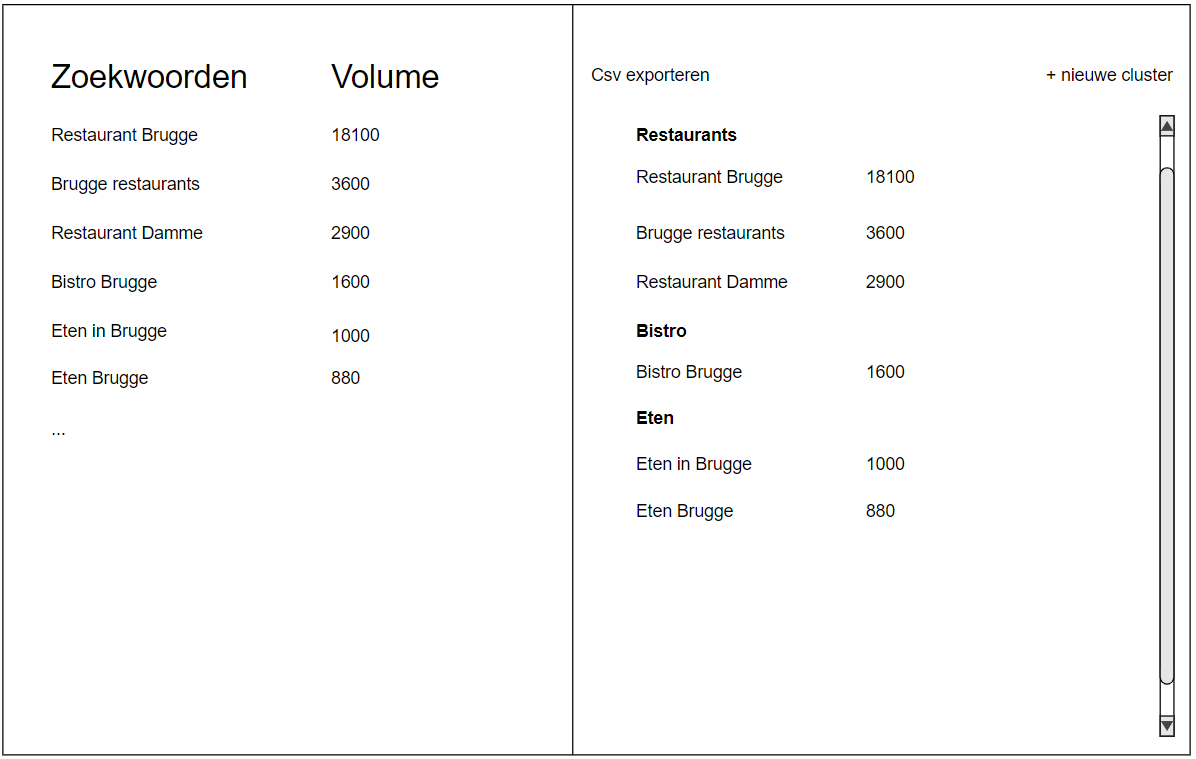
\includegraphics[width=\linewidth]{img/Mockup2.png}
\caption{Screenshot van mock-up 2}
\end{figure}

Er staat een overzichtelijk scherm met alle zoekwoorden aan de linkerkant en een optie om clusters te creëren aan de rechterkant. Bij dit scherm krijgt de gebruiker de optie om een zoekwoord te selecteren en in de juiste cluster toe te voegen (of om eerst een nieuwe cluster aan te maken). 

Tot slot kan je als gebruiker al deze clusters met hun zoekwoorden exporteren naar een Csv- of Excel-bestand om verder te gebruiken. 

Op deze manier verricht je veel minder handmatig werk dan wanneer je alle zoekwoorden apart gaat kopiëren en plakken in een Spreadsheet of Excel-bestand. 

Er wordt dus vanaf nul een tool geprogrammeerd die voor een deel gebaseerd is op een bestaande tool. 

\section{Werking}
\label{ch: Werking}

\subsection{DataForSEO API}
\label{ch: DataForSEO API}

Om zoekwoordsuggesties en zoekvolumes te krijgen werd er gewerkt via een externe API. Via het online platform, DataForSEO, kon deze API geïntegreerd worden in het programma. 

Het programma is geschreven in de programmeertaal Java (Netbeans). Via deze documentatie, \textcite{DATAFORSEO}, wordt er aangetoond hoe de API in Java (Netbeans) geïmplementeerd kan worden. 

In de API-code kan je zelf verschillende elementen instellen: het zoekwoord waarvan je suggesties wil krijgen, het land, de taal en hoeveel zoekwoordsuggesties je wilt per zoekwoord. Deze code geeft dan gegevens zoals het zoekwoord, volume, ... terug in JSON-formaat. 

Dit is een voorbeeld van een JSON-output: 

\begin{figure}[h!]
\centering
\includegraphics[width=\linewidth]{img/jsoncode.PNG}
\caption{Voorbeeld van jsoncode}
\end{figure}

Bij de sectie 'related' worden de gerelateerde zoekwoorden (of zoekwoordsuggesties) gegeven. De meest relevante elementen die gebruikt worden zijn 'key' en 'search\_volume' omdat we bij de output enkel deze twee nodig hebben. 

Om de JSON-code te gebruiken in de applicatie, werd deze omgezet naar een Arraylist die door een MVC-applicatie (Model-View-Controller) gebruikt werd. 

\subsection{Model-View-Controller-Applicatie}
\label{ch: Model-View-Controller-Applicatie}

MVC-patroon staat voor Model-View-Controller-patroon. Dit patroon wordt gebruikt om de 'taken' te scheiden van de applicatie. 

'Model' staat voor een object met gegevens. Het kan ook een logica hebben om de controller bij te werken wanneer de gegevens veranderen. 

'View' vertegenwoordigt de visualisatie van de gegevens van het model. Het programma maakt gebruik van JavaFX Scenebuilder om het View-gedeelte op te bouwen. 

'Controller' werkt zowel op 'model' als op de 'View'. Het stuurt de datastroom naar het modelobject en werkt de weergave bij telkens wanneer de gegevens worden gewijzigd.

\subsubsection{Model-klasse}
\label{ch: Model-klasse}

Het JSON-bestand dat verkregen wordt via de API van DataForSEO wordt (in de Model-klasse) omgezet in een Arraylist (bijvoorbeeld met de volgende output: ["restaurant Brugge", 340; "Bistro Brugge", 250].)

Deze Arraylist wordt omgezet naar een Observablelist om te kunnen communiceren met de Controller (die aan de View gekoppeld is). 

\subsubsection{View-klassen}
\label{ch: View-klassen}

Er zijn in het programma twee View-klassen. Met behulp van het programma JavaFX Scenebuilder werden de twee schermen opgebouwd.

De eerste klasse is het startscherm waarbij de gebruiker drie waarden moet meegeven: de taal, het land en het zoekwoord waarvan er suggesties moeten gegeven worden. 

Het startscherm van de applicatie ziet er als volgt uit (opgemaakt in JavaFX Scenebuilder): 

\begin{figure}[h!]
\centering
\includegraphics[width=\linewidth]{img/keywordtoolscherm1.PNG}
\caption{Scherm 1 van de zelfgemaakte keywordtool}
\end{figure}

In het tekstvak (onder 'geef zoekwoord in:') kan je een zoekwoord ingeven zoals 'Restaurant Brugge' om zoekwoordsuggesties te krijgen. In de eerste dropdownlist kan je een land selecteren (België of Nederland) om het zoekwoordvolume te krijgen voor een specifiek land. In de rechtste dropdownlist (Onder 'Geef taal in:') kan je de taal kiezen van het zoekwoord, Nederlands of Engels. 

Deze droe waarden worden vervolgens (door op de knop 'vind zoekwoorden' te klikken) door middel van setters automatisch in de API-code geïntegreerd. Uit deze API-code wordt meteen de nodige JSON-code gegenereerd. 

De JSON-code wordt omgezet in leesbare taal voor de controller en er wordt een tableview gegenereerd met twee kolommen: de zoekwoorden met het maandelijks gemiddeld zoekvolume van de laatste 12 maanden (voor het gekozen land en taal). 

Nadat er op de knop 'Vind zoekwoorden' geklikt is heeft het scherm een linker- en rechterkant. Aan de linkerkant wordt een tableview (lijst) gegenereerd met de zoekwoordsuggesties en het bijhorende zoekvolume. 

\begin{figure}[h!]
\centering
\includegraphics[width=\linewidth]{img/scherm2linkerkant.PNG}
\caption{Scherm 2, linkerkolom van de zelfgemaakte tool}
\end{figure}

Bovenaan is er een knop om terug te keren naar de startpagina. De tableview van de linkerkolom wordt dan automatisch terug geledigd. 

Er staat een knop ( >> ) om de zoekwoorden van links naar rechts over te brengen. 

In de rechterkolom staat een tabel om de zoekwoorden en het zoekvolume van de linkerkolom in over te brengen. De tabel kan onderverdeeld worden in verschillende secties om de zoekwoorden en het zoekvolume te groeperen in clusters. 

Om een nieuwe sectie (of cluster) aan te maken, geef je de naam in van de sectie en druk je op de knop '+ cluster'. Binnen die sectie kan je dan zoekwoorden toevoegen.

Er staat een knop ( << ) om de zoekwoorden van de rechterkant terug over te brengen naar de linkerkant indien het zoekwoord toch niet nodig is in de lijst. 

Bovenaan staat een knop om de tableview te exporteren naar een Excel-bestand dat uiteindelijk kan geleverd worden aan de klant. 


\subsubsection{Controller-klassen}
\label{ch: Controller-klassen}

De Java-Applicatie heeft twee controller-klassen. Het startscherm heeft een controller-klasse die de ingevoerde waarden doorstuurt naar de API-klasse. Door middel van setters worden de waarden (zoekwoord, land en taal) correct ingesteld en wordt de JSON-code gegenereerd. 

Nadat de JSON-code is omgezet naar een Arraylist, worden de gegevens in een Tableview omgezet. De tweede controller-klasse is verantwoordelijk voor de Tableviews (linker- en rechterkant). 

\begin{figure}[h!]
\centering
\includegraphics[width=\linewidth]{img/scherm2linkerkant.PNG}
\caption{Scherm 2, rechterkolom van de zelfgemaakte tool}
\end{figure}

% Voeg hier je eigen hoofdstukken toe die de ``corpus'' van je bachelorproef
% vormen. De structuur en titels hangen af van je eigen onderzoek. Je kan bv.
% elke fase in je onderzoek in een apart hoofdstuk bespreken.

%\input{...}
%\input{...}
%...

\chapter{Conclusie}
\label{ch:conclusie}



%%=============================================================================
%% Bijlagen
%%=============================================================================

\appendix

%%---------- Onderzoeksvoorstel -----------------------------------------------

\chapter{Onderzoeksvoorstel}

Het onderwerp van deze bachelorproef is gebaseerd op een onderzoeksvoorstel dat vooraf werd beoordeeld door de promotor. Dat voorstel is opgenomen in deze bijlage.

% Verwijzing naar het bestand met de inhoud van het onderzoeksvoorstel
%---------- Inleiding ---------------------------------------------------------

\section{Introductie} % The \section*{} command stops section numbering
\label{sec:introductie}

Het probleem is bij vele SEO tools dat ze redelijk duur geprijsd zijn en er betere alternatieven bestaan op de markt. Hierin zal een vergelijking gemaakt worden tussen verschillende tools op vlak van prijs, soort tool en prestatie. De reden van dit onderzoek is omdat WISEO op die manier commercieel meer opdrachten kan binnenhalen door beter onderzoek te kunnen voeren aan een goedkoper tarief. De doelstelling is dus om de volgende onderzoeksvragen te beantwoorden: Welke seo tools kunnen best als hulpmiddel gebruikt worden voor meer zichtbaarheid in zoekmachines? (Hierbij wordt gekeken naar welke tools de meeste informatie weergeven zodat SEO'ers zoals WISEO dit kunnen implementeren) Wat is duur voor een SEO tool (vergelijkende studie)? Hoe gebeurt het uitwerken en verbeteren van een keyword tool?

%---------- Stand van zaken ---------------------------------------------------

\section{Literatuurstudie}
\label{sec:Literatuurstudie}

In dit domein zijn er al gelijkaardige onderzoeken te vinden in de vorm van blogposts. Om te beginnen wordt er gerefereerd naar een artikel over keywordplanners, \textcite{BKRT2018}. Met behulp van deze tools zullen de beste functionaliteiten (dit zal pas duidelijk zijn na een onderzoek) gekozen worden om dan een eigen zoekwoorden tool te maken.


Er worden in de referenties nog 2 andere artikels vermeld die gaan over de beste SEO tools, \textcite{SEO13}, en de volledige lijst van SEO tools 2018, \textcite{SEOCOMPLETE}. Deze blogposts hebben relevantie tot het onderzoek die hier zal gevoerd worden in de zin dat er ook een vergelijking zal gebeuren tussen meerdere tools. De meeste tools zijn trials die na verloop van tijd betalend zijn en duur kunnen oplopen. WISEO, als ervaren SEO specialisten, zegt hierbij dat er nog te weinig onderzoek wordt gedaan naar tools die gelijkaardig werken en een goedkoper (de studie zal ook uitwijzen wat goedkoop is en wat niet) alternatief vormen. 

% Voor literatuurverwijzingen zijn er twee belangrijke commando's:
% \autocite{KEY} => (Auteur, jaartal) Gebruik dit als de naam van de auteur
%   geen onderdeel is van de zin.
% \textcite{KEY} => Auteur (jaartal)  Gebruik dit als de auteursnaam wel een
%   functie heeft in de zin (bv. ``Uit onderzoek door Doll & Hill (1954) bleek
%   ...'')

%---------- Methodologie ------------------------------------------------------
\section{Methodologie}
\label{sec:methodologie}

Er zal een vergelijkende studie plaatsvinden tussen meerdere SEO tools die gemeten en ingedeeld zullen worden op basis van prijs, soort tool (er zijn tools met verschillende doeleinden zoals: keywordresearch, linkbuilding, ranking, content optimization en technical SEO tools) en de prestatie (wat levert de meeste en duidelijkste informatie op die SEO'ers het best kunnen gebruiken) ervan. Hieruit zal er vooral duidelijkheid blijken uit welke tools de meeste info kan worden gevonden per SEO onderdeel (zoekwoordenonderzoek, SEO audit opstellen, enz...). De experimenten zullen onder andere bestaan uit: zoekwoordenonderzoektools vergelijken om te kijken welke het beste resultaat levert, vergelijking bij audit tools om zoveel mogelijk info te weten te komen, enz... Voor het onderzoek en op vraag van WISEO wordt ook een eigen tool gemaakt op vlak van zoekwoordenonderzoek om aan te tonen dat er nog verbetering mogelijk is bij sommige tools. Er zullen voornamelijk tools getest en vergeleken worden die vermeld staan in de opgesomde artikelen bij referenties.

%---------- Verwachte resultaten ----------------------------------------------
\section{Verwachte resultaten}
\label{sec:verwachte_resultaten}

Als resultaat wordt er verwacht dat er tools een beter alternatief vormen voor bepaalde tools die momenteel meest gebruikt worden door KMO's en WISEO. Er moet een duidelijk beeld worden gevormd welke de beste zijn zodat WISEO hier gebruik van kan maken. Tussen de verschillende soorten tools (wat je ermee kan bereiken) wordt een vergelijking gemaakt waarbij rekening gehouden wordt met de kost en prestaties (welke het meeste en duidelijke info levert). Als laatste wordt er een eigen keyword research tool geschreven die in de toekomst gebruikt kan worden.

%---------- Verwachte conclusies ----------------------------------------------
\section{Verwachte conclusies}
\label{sec:verwachte_conclusies}

De verwachte conclusie is dat er een duidelijke lijst zal worden weergegeven tussen de prijs/kwaliteit van verscheidene tools. Verder wordt er verwacht dat er vele tools zijn met te weinig functionaliteit en deze dus beter vervangen worden door andere, betere SEO tools. In de artikelen (zie referenties) worden soms ook dure tools vermeld. Dit onderzoek zal duidelijk maken dat dit niet altijd hoeft. Als laatste conclusie wordt er verwacht dat het mogelijk is om een eigen keyword tool te implementeren die aantoont dat er nog mogelijkheid is tot verbetering op vlak van SEO tools.




%%---------- Andere bijlagen --------------------------------------------------
% TODO: Voeg hier eventuele andere bijlagen toe
%%%%%%%%%%%%%%%%%%%%%%%%%%%%%%%%%%%%%%%%%%
% LaTeX-sjabloon voorstel onderwerp Bachelorproef
% HoGent Bedrijf en Organisatie, opleiding toegepaste informatica
% 
% Gebaseerd op ``Stylish Article'' class
% Version 2.1 (1/10/15)
%
% This template has been downloaded from:
% http://www.LaTeXTemplates.com
%
% Original author:
% Mathias Legrand (legrand.mathias@gmail.com)
% With extensive modifications by:
% Vel (vel@latextemplates.com)
%
% License:
% CC BY-NC-SA 3.0 (http://creativecommons.org/licenses/by-nc-sa/3.0/)
%
%%%%%%%%%%%%%%%%%%%%%%%%%%%%%%%%%%%%%%%%%

\NeedsTeXFormat{LaTeX2e}
\ProvidesClass{voorstel}
\RequirePackage{ifthen}
\RequirePackage{calc}
\AtEndOfClass{\RequirePackage{microtype}}
\DeclareOption*{\PassOptionsToClass{\CurrentOption}{article}}
\ProcessOptions*
\LoadClass{article}
\RequirePackage{ifpdf}      % Needed to pick between latex and pdflatex

%----------------------------------------------------------------------
%  FONTS & COLORS
%----------------------------------------------------------------------

\RequirePackage{times}      % Loads the Times-Roman Fonts
\RequirePackage{mathptmx}   % Loads the Times-Roman Math Fonts

\RequirePackage{xcolor}
\definecolor{color1}{RGB}{0,147,208} % Color of the article title and sections
\definecolor{color2}{RGB}{0,20,20} % Color of the boxes behind the abstract and headings

%----------------------------------------------------------------------
%  VARIOUS USEFUL PACKAGES
%----------------------------------------------------------------------

\RequirePackage[utf8]{inputenc}
\RequirePackage{amsmath,amsfonts,amssymb}
\RequirePackage{graphicx}
\RequirePackage{booktabs}
\RequirePackage{csquotes}
\RequirePackage[english,dutch]{babel}
\usepackage{hyperref}                      % hyperlinks
\hypersetup{hidelinks,colorlinks,breaklinks=true,urlcolor=black,citecolor=color2,linkcolor=color2,bookmarksopen=false,pdftitle={Title},pdfauthor={Author}}

%----------------------------------------------------------------------
%  MARGINS
%----------------------------------------------------------------------

\RequirePackage[left=2cm,%
right=2cm,%
top=2.25cm,%
bottom=2.25cm,%
headheight=11pt,%
letterpaper]{geometry}%

%----------------------------------------------------------------------
%  FIGURES AND TABLES CAPTIONS
%----------------------------------------------------------------------

\RequirePackage[labelfont={bf,sf,small},%
labelsep=period,%
justification=raggedright]{caption}
\setlength{\abovecaptionskip}{0pt}
\setlength{\belowcaptionskip}{0pt}

%----------------------------------------------------------------------
%  PAGE HEADER
%----------------------------------------------------------------------

\RequirePackage{fancyhdr}  % Needed to define custom headers/footers
\RequirePackage{lastpage}  % Number of pages in the document
\pagestyle{fancy}          % Enables the custom headers/footers
% Headers
\lhead{\includegraphics[height=1.1cm]{FBO-NL.jpg}}%
\chead{}%
\rhead{\small\sffamily\bfseries\@PaperTitle\  --- \thepage/\pageref{LastPage}}
% Footers
\lfoot{}%
\cfoot{}%
\rfoot{}%
\renewcommand{\headrulewidth}{0pt}% % No header rule
\renewcommand{\footrulewidth}{0pt}% % No footer rule

%----------------------------------------------------------------------
%  SECTION/SUBSECTION/PARAGRAPH SET-UP
%----------------------------------------------------------------------

\RequirePackage[explicit]{titlesec}
\titleformat{\section}
  {\color{color1}\large\sffamily\bfseries}
  {}
  {0em}
  {\colorbox{color2!10}{\parbox{\dimexpr\linewidth-2\fboxsep\relax}{\centering\arabic{section}. #1}}}
  []
\titleformat{name=\section,numberless}
  {\color{color1}\large\sffamily\bfseries}
  {}
  {0em}
  {\colorbox{color2!10}{\parbox{\dimexpr\linewidth-2\fboxsep\relax}{\centering#1}}}
  []
\titleformat{\subsection}
  {\color{color1}\sffamily\bfseries}
  {\thesubsection}
  {0.5em}
  {#1}
  []
\titleformat{\subsubsection}
  {\sffamily\small\bfseries}
  {\thesubsubsection}
  {0.5em}
  {#1}
  []
\titleformat{\paragraph}[runin]
  {\sffamily\small\bfseries}
  {}
  {0em}
  {#1}
\titlespacing*{\section}{0pc}{3ex \@plus4pt \@minus3pt}{5pt}
\titlespacing*{\subsection}{0pc}{2.5ex \@plus3pt \@minus2pt}{0pt}
\titlespacing*{\subsubsection}{0pc}{2ex \@plus2.5pt \@minus1.5pt}{0pt}
\titlespacing*{\paragraph}{0pc}{1.5ex \@plus2pt \@minus1pt}{10pt}

%----------------------------------------------------------------------
%  TABLEOFCONTENTS SET-UP
%----------------------------------------------------------------------
\newlength{\tocsep}
\setlength\tocsep{1.5pc} % Sets the indentation of the sections in the table of contents
\setcounter{tocdepth}{3} % Three levels in the table of contents section: sections, subsections and subsubsections

\usepackage{titletoc}
\contentsmargin{0cm}
\titlecontents{section}[\tocsep]
  {\addvspace{4pt}\small\bfseries\sffamily}
  {\contentslabel[\thecontentslabel]{\tocsep}}
  {}
  {\hfill\thecontentspage}
  []
\titlecontents{subsection}[\tocsep]
  {\addvspace{2pt}\sffamily}
  {\contentslabel[\thecontentslabel]{\tocsep}}
  {}
  {\ \titlerule*[.5pc]{.}\ \thecontentspage}
  []
\titlecontents*{subsubsection}[\tocsep]
  {\footnotesize\sffamily}
  {}
  {}
  {}
  [\ \textbullet\ ]

%----------------------------------------------------------------------
%  MULTIPLE AUTHOR SET
%----------------------------------------------------------------------

\newcount\@authcnt
\newcount\@tmpcnt\@tmpcnt\z@

\def\@affiliation{%
  \ifnum\@tmpcnt<\@authcnt
   \global\advance\@tmpcnt1
    \raggedright \csname @auth\romannumeral\the\@tmpcnt\endcsname\hfill\\%
   \let\next\@affiliation \vskip1pt
  \else
   \let\next\relax
  \fi
\next}

\newcommand{\affiliation}[1]{%
    \global\advance\@authcnt1
    \expandafter\gdef\csname @auth\romannumeral\the\@authcnt\endcsname
    {#1}}

%----------------------------------------------------------------------
%  LIST CONTROL
%----------------------------------------------------------------------

\RequirePackage{enumitem}
\setlist{nolistsep} % Uncomment to remove spacing between items in lists (enumerate, itemize)

%----------------------------------------------------------------------
%  ABSTRACT+AUTHOR FRAME
%----------------------------------------------------------------------

\newcommand{\PaperTitle}[1]{\def\@PaperTitle{#1}}
\newcommand{\PaperType}[1]{\def\@PaperType{#1}}
\newcommand{\Archive}[1]{\def\@Archive{#1}}
\newcommand{\Authors}[1]{\def\@Authors{#1}}
\newcommand{\JournalInfo}[1]{\def\@JournalInfo{#1}}
\newcommand{\Abstract}[1]{\def\@Abstract{#1}}
\newcommand{\Keywords}[1]{\def\@Keywords{#1}}
\newcommand{\CoPromotor}[1]{\def\@CoPromotor{#1}}

% ---------------------------------------------------------------------
\setlength{\columnsep}{0.55cm} % Distance between the two columns of text
\setlength{\fboxrule}{0.75pt} % Width of the border around the abstract

\renewcommand{\@maketitle}{%
\twocolumn[{%
\thispagestyle{empty}%
\vskip-36pt%
{\raggedleft\small\sffamily\bfseries\@JournalInfo\\\@Archive\par}%
\vskip20pt%
{\raggedright\color{color1}\sffamily\bfseries\fontsize{20}{24}\selectfont \@PaperTitle\\}%
{\raggedright\color{color1}\sffamily\bfseries\fontsize{13}{15.6}\selectfont \@PaperType\par}%
\vskip10pt%
{\raggedright\color{color1}\sffamily\fontsize{12}{16}\selectfont  \@Authors\par}%
\vskip18pt%
\fcolorbox{color1}{white}{%
\parbox{\textwidth-2\fboxsep-2\fboxrule}{\centering%
\colorbox{color2!10}{%
\parbox{\textwidth-4\fboxsep-2\fboxrule}{%
\sffamily\textbf{\abstractname}\\\@Abstract%
\ifx\@Keywords\@empty%
\else%
\\[4pt]\textbf{\keywordname}\\\@Keywords%
\fi%
\ifx\@CoPromotor\@empty%
\else%
\\[4pt]\textbf{Co-promotor}\\\@CoPromotor%
\fi%
}%
}%
\vskip4pt%
\begingroup%
\raggedright\sffamily\small%
\footnotesize\@affiliation\par%
\endgroup%%
}%
}%
\vskip25pt%
}]%
}

%----------------------------------------------------------------------
%  REFERENCES
%----------------------------------------------------------------------

\RequirePackage[backend=biber,style=apa]{biblatex}
\DeclareLanguageMapping{dutch}{dutch-apa}
\addbibresource{voorstel.bib}



%%---------- Referentielijst --------------------------------------------------

\printbibliography[heading=bibintoc]
%\addbibresource{bachproef-tin.bib}
%\addcontentsline{toc}{chapter}{\textcolor{maincolor}{\IfLanguageName{dutch}{Bibliografie}{Bibliography}}}

\end{document}
